\documentclass[aps,floatfix,prd,superscriptaddress,twocolumn]{revtex4-1}
% Intended to be built with pdflatex, using the REVTEX 4.1 package.
% Template taken from FermiLab APS Journal template.

% packages
\usepackage{amssymb}              % for \gtrsim ...
\usepackage{amsmath}              % for \text, align, split ...
\usepackage{color}                % for colorful margin notes
\usepackage[mathscr]{euscript}    % for \mathscr
\usepackage{float}                % for better control of figure placement
\usepackage{graphicx}             % for \includegraphics
\usepackage{hyperref}             % for \url and \href
\usepackage{listings}             % for typesetting code with \lstinline
\usepackage{tabularx}             % for tabularx

% commands/initialization
\hyphenation{ALPGEN} % avoid incorrect hyphenation
\hyphenation{EVTGEN} % ''
\hyphenation{PYTHIA} % ''
\lstset{basicstyle=\ttfamily} % define \lstinline for inline code snippet

\newcommand{\todo}[1]{\marginpar{\tiny{\textcolor{red}{#1}}}}
%\renewcommand\todo[1]{} % if you wish to hide all todo notes

% force all figures to be placed right where they are in the text
\floatplacement{figure}{H}

% *******************************************************************************
\begin{document}

\widetext
\leftline{Compiled \today}
\leftline{To be submitted to PRD}

\title{Elastic Scattering in General Relativistic Ray Tracing for Neutrinos}

\author{M.\ Brett Deaton}
\email{mbdeaton@ncsu.edu}
\affiliation{Joint Institute for Nuclear Astrophysics,
  Michigan State University, East Lansing, MI 48824, USA}
\affiliation{Department of Physics,
  North Carolina State University, Raleigh, NC 27695, USA}

\author{Evan O'Connor}
\affiliation{Department of Physics,
  North Carolina State University, Raleigh, NC 27695, USA}

\author{Andy Bohn}
\affiliation{Center for Radiophysics and Space Research,
  Cornell University, Ithaca, NY 14853, USA}

\author{Jerred Jesse}
\affiliation{Department of Physics \& Astronomy,
  Washington State University, Pullman, WA 99164, USA}

\author{Francois Foucart}
\affiliation{Lawrence Berkeley National Laboratory,
  1 Cyclotron Rd., Berkeley, CA 94720, USA}

\author{Matthew D.\ Duez}
\affiliation{Department of Physics \& Astronomy,
  Washington State University, Pullman, WA 99164, USA}

\author{G.\ C.\ McLaughlin}
\affiliation{Department of Physics,
  North Carolina State University, Raleigh, NC 27695, USA}

% *******************************************************************************

\begin{abstract}
  We present a covariant ray tracing algorithm for computing high-resolution
  neutrino distributions in general numerical spacetimes with hydrodynamical
  sources.
  Our formulation treats the very important effect of
  elastic scattering of neutrinos off of nuclei and nucleons
  (changing the neutrino's direction but not energy)
  by incorporating estimates of the background neutrino fields.
  These background fields may be taken from a low-order moment simulation
  or be ignored entirely, in which case the method
  reduces to a standard state-of-the-art ray tracing formulation.
  It handles radiation in regimes spanning optically thick to optically thin.
  We test the new code, highlight its strengths and weaknesses, and
  apply it to simulations of neutron star mergers to
  compute neutrino fluxes as a function of energy and emission angle.
\end{abstract}

\maketitle

\section{Introduction}
Neutrinos are one of the dominant energy transport phenomena at play in
neutron star mergers, heating, cooling, and pushing the disrupted nuclear
matter.
In addition, they change the composition of the matter via charged current
interactions.
Because neutrinos scatter over length scales both large and small with
respect to fluid scales, accurate models require a neutrino treatment that
respects the freedom of neutrino distribution functions to vary
drastically from simple geometric distributions in thermodynamic equilibrium.

This is a challenging task in the environment of a merger,
which generally lacks any spatial symmetries so that fully general
seven-dimensional solutions to the Boltzmann Equation are not feasible.
Leakage approximations
\citep{deat2013-leakage, pere2016-asl, radi2016-dynamical}
\todo{cite others}
capture the qualitative effects of neutrinos on the matter, but
provide extremely limited information about the neutrino field itself.
\todo{discuss mc more clearly}
Monte Carlo methods \citep{abdi2012-monte_carlo, rich2015-monte_carlo}
are an excellent tool require large computational resources because of
their global treatment of the problem.

The state of the art today couples radiation and matter with a truncated
moment formalism
\citep{shib2011-truncated_moment, fouc2015-m1_nsbh, fouc2016-m1_nsns,
  just2015-m1_code},
\todo{cite others}
evolving the zeroth- and first-angular moments of the distribution function
(the energy density and flux respectively) representing the zeroth-energy moment
of the radiation field (the total energy).
This method, commonly called M1 transport, was formulated by
\cite{thor1981-truncated_moment, shib2011-truncated_moment}
and has been applied for example in \cite{ramp2002-truncated_moment,
  card2013-truncated_moment, fouc2015-m1_nsbh, ocon2015-gr1d_with_nu}.
Recently, \cite{fouc2016-m1_evolve_n} have expanded their M1 transport code
to also evolve the number densities of neutrinos,
providing total and average energies throughout the simulated volume.
Even so, with M1 transport codes only evolving two angular moments
and one or two energy moments,
we can extract only limited angular and spectral information
from the neutrino fields.

%\subsubsection*{What physics problems do we want to address?}
But many interesting unsolved problems require an accurate model of the neutrino
spectra and angular distributions.
With a model of the neutrino emission from a merger we can
1) examine neutrino effects on the nucleosynthesis of the ejected material
\citep{surm2011-nickel_56, robe2016-sph_nu_nucleo},
2) explore the rich flavor oscillation physics likely to occur
\citep{malk2012-mnr_1, malk2015-mnr_2, malk2016-mnr_3, zhu2016-mnr_nsns_remnant,
  vaan2016-uncovering_mnr},
3) improve closure relations used in M1 transport schemes
\citep{ramp2002-truncated_moment, shib2011-truncated_moment,
  card2013-truncated_moment, fouc2015-m1_nsbh, ocon2015-gr1d_with_nu}, and
4) study possible jet formation due to neutrino annihilation
\citep{ruff1999-nunubar_nsns, asan2000-nunubar, birk2007-nunubar,
  hari2010-gr_nunubar_collapsar, zala2011-nunubar, leng2014-nunubar}.

%\subsubsection*{Why ray tracing?}
In this work we present a ray tracing method to compute neutrino distribution
functions from state-of-the-art general relativistic M1 transport
hydrodynamics simulations.
We choose ray tracing because it is conceptually simple, numerically cheap,
and easily extends to high resolution in energy and angle.

With a ray tracing method we approach radiation transport from the perspective
of a single observer at a spacetime event $x_o^\alpha$.
Our goal is to compute the distribution function
$f^{\nu_\sigma}(x_o^\alpha;p_\beta)$, or the amount of neutrino radiation
of species $\nu_\sigma\in\{\nu_{\{e,\mu,\tau\}},\bar{\nu}_{\{e,\mu,\tau\}}\}$
with momentum $p_\beta$ impinging on $x_o^\alpha$.
To do so we trace a geodesic trajectory from $x_o^\alpha$ in the backwards
direction $-p_\beta$ to sample the incoming radiation along that line of sight.
By tracing a family of rays intersecting $x_o^\alpha$ we build up a
picture of the distribution function there.
And by sampling many observation points we construct a global picture
of $f^{\nu_\sigma}(x^\alpha;p_\beta)$.

The ray tracing framework
is conceptually simple because it solves the equation of radiation
transport (Eqn.~\ref{eqn:boltzmann}) along characteristics,
reducing it to a one-dimensional ordinary differential equation.
It is numerically cheap because it confines computations of
$f^{\nu_\sigma}(x_o^\alpha;p_\beta)$ to the past light-cone of $x_o^\alpha$,
with the history of that light-cone truncated at large optical depth.
\todo{state scaling $\mathscr{O}(n)$?}
And it easily extends to high resolution in energy and angle by simply
increasing the number of rays sampled.

%\subsubsection*{What is new and better about this ray tracing formulation?}
Several ray tracing formulations for radiation transport already exist.
Most formulations assume an analytic spacetime metric
\citep{birk2007-nunubar, hari2010-gr_nunubar_collapsar, kova2011-gr_ray_tracing}.
And many make the simplifying assumption of blackbody emission from a
neutrinosurface \citep{birk2007-nunubar, kova2011-gr_ray_tracing},
limiting them to equilibrium, optically thick configurations.
Current state-of-the-art ray tracing formulations avoid the assumption of
blackbody spectra by integrating a local emissivity along each geodesic
(e.g. \cite{hari2010-gr_nunubar_collapsar} for neutrinos and
\cite{youn2012-gr_radiative_transfer} for photons).
But no formulations to date account for the important scattering and pair
processes outlined in Tab.~\ref{tab:neutrino_processes}.

We build upon existing ray tracing formulations
by eschewing any assumptions about the spacetime geometry,
integrating local emissivities,
and including elastic scattering in the integration along each geodesic.
To incorporate scattering processes in our method, we employ estimates of the
lowest-order moment of the neutrino distribution function
computed in an M1 transport simulation.
If moments are not available either from
an M1 transport evolution or a trustworthy analytical estimate,
our method reduces to the current state-of-the-art ray tracing method,
neglecting scattering.

%\subsubsection*{Why does a covariant formulation matter?}
We formulate our ray tracing equations covariantly---free from
assumptions about the spacetime geometry or coordinates. This is essential
because we want to apply the method as a postprocessing step using
time snapshots of data computed from general relativistic evolutions.
The spacetime represented in these snapshots is not analytic (i.e. Kerr).
And even in configurations that are described well by the Kerr metric
(e.g. a low-mass disk around a massive black hole),
the evolution coordinates are unlikely to present the metric in
a familiar analytic form.
This is because integrating the Einstein Equations often requires complicated,
time-dependent gauge conditions
\citep{lind2007-gen_harmonic, fouc2013-compactness_and_spin}.

%\subsubsection*{Why do scattering and pair processes matter?}
Elastic scattering (see Tab.~\ref{tab:neutrino_processes}) can signicantly
modify neutrino distributions in angle and dilute the emitted spectrum over a
larger emitting surface \citep{pere2016-asl}.
This is especially pronounced in the case of heavy-lepton neutrinos.
\todo{cite}
Inelastic scattering and pair processes can introduce further modifications.
Any phenomena that involve neutrino-neutrino interactions,
for example neutrino oscillations and neutrino-antineutrino annihilation,
\todo{cite}
depend sensitively on the angular distribution.
And spectral changes can strongly affect the nucleosynthesis
occuring in the ejected and irradiated material.
\todo{justify these statements}
The ray tracing method we present in this paper captures the dominant effects
of elastic scattering, while leaving the physics of inelastic scattering and
pair processes for later work.

%\subsubsection*{In what ways is this method limited?}
Ray tracing is ideally suited to problems requiring detailed knowledge of
radiation distribution functions over small regions of spacetime:
for example along a matter or radiation trajectory,
or over a small volume outside a source.
But the method becomes computationally burdensome when the inquiry extends
to large volumes of spacetime.

More fundamentally, though, ray tracing is limited by its naive
treatment of the Boltzmann Equation (Eqn.~\ref{eqn:boltzmann}),
a treatment which essentially decouples different neutrino momenta and species.
\todo{clarify how momenta are decoupled}
When we're solving for $f^{\nu_\sigma}(x^\alpha;p_\beta)$, we have no
information about $f^{\nu_\sigma}(x^\alpha;p'_\beta)$, and
$f^{\bar{\nu}_\sigma}(x^\alpha;p'_\beta)$, which are essential ingredients
for the source terms of the Boltzmann Equation describing the creation and
destruction of neutrinos due to the interaction processes described in
Tab.~\ref{tab:neutrino_processes}.

In this paper we outwit this limitation by incorporating coupled source terms
that depend on either previously-evolved or analytical
estimates of the neutrino fields.
We also retain the freedom to drop the coupling terms, in which case our method
becomes similar to existing state-of-the-art ray tracing methods.
Our method is not a standalone radiation transport scheme,
but serves as the final component of a hybrid scheme,
piggy-backing on a lower-order radiation transport method as a
post-processing step.

\subsubsection*{Outline}
In Sec.~\ref{sec:formulation} we derive the ray tracing equations from the
Boltzmann Equation and describe our numerical scheme.
In Sec.~\ref{sec:tests} we present tests of the code.
In Sec.~\ref{sec:applications} we present several applications
in the dynamical environment following the merger of two neutron stars:
computing neutrino spectra as a function of observer's angle,
computing the self-interaction potential descriptive of flavor evolution
in high-neutrino-density environments,
and computing the energy dumped into jet-forming electron-positron
pairs via neutrino-antineutrino annihilation.

Greek tensor indices ($\alpha, \beta, ...$) range over all four coordinates,
whereas Latin indices ($i, j, ...$) range over the spatial coordinates 1--3.
We use naturalized units in which $\hbar=c=1$.
And for most of the remainder of this article we suppress neutrino species label
$\nu_\sigma$ since the formulation is general to any species.
Where we do reference particular species we use the three categories
$\nu_e$, $\bar{\nu}_e$, and
$\nu_x=\left\{\nu_\mu,\bar{\nu}_\mu,\nu_\tau,\bar{\nu}_\tau\right\}$.

\section{Ray tracing formulation}
\label{sec:formulation}
The neutrino distribution function, $f(x^\alpha; p_\beta)$ is an invariant
quantity counting the number of neutrinos in a given six-volume of phase
space centered on $(x^\alpha,p_\beta)$.
The phase space volume elements are defined with respect to a fiducial
observer passing through event $x^\alpha$ with velocity $u^\alpha$:
\begin{align}
  \label{eqn:dV}
  dV & \equiv \sqrt{-\psi} \, dx \, dy \, dz \, u^t \\
  \label{eqn:dP}
  dP & \equiv \frac{1}{\sqrt{-\psi}} \, dp_x \, dp_y \, dp_z \,
  \frac{\varepsilon}{p^t},
\end{align}
where $\psi$ represents the determinant of the spacetime metric,
the index $t$ indicates the time-component of the given four-vector, and
\begin{equation}
  \label{eqn:varepsilon}
  \varepsilon \equiv -p_\mu u^\mu
\end{equation}
is the neutrino energy measured by our observer.
The number of particles in a given six-volume is
\begin{equation}
  dN=\frac{g}{(2\pi)^3}\,f\,dV\,dP,
\end{equation}
where $g$ counts the number of spin states accessible to the
particles ($g=1$ for neutrinos), and $f$ is the distribution function.
Each of $dV$, $dP$, $dN$, and $f$ are spacetime invariants
\citep{debb2009-gr_boltzmann_1, debb2009-gr_boltzmann_2, lind1966-gr_boltzmann}.

We may decompose the neutrino momentum like
\begin{equation}
  \label{eqn:def_momentum}
  p_\beta = \varepsilon (u_\beta + \ell_\beta),
\end{equation}
with $\ell_\beta$ the direction normal subject to the constraints
$u^\alpha \ell_\alpha = 0$ and $\ell^\alpha \ell_\alpha=1$.
With this decompositon we can write the arguments to the distribution function
$f(x^\alpha;\varepsilon,\ell_\beta)$.

Because $\ell_\beta$ is subject to two constraints
(normalization and orthogonality to the observer's velocity)
it has two degrees of freedom; we make this explicit by defining its
spatial cartesian components with respect to spherical polar angles
\begin{equation}
  \label{eqn:def_direction}
  \ell_\alpha \rightarrow
  q (s,\sin a \cos b,\sin a\sin b,\cos a),
\end{equation}
with $q$ and $s$ functions of $a$ and $b$.
Now our symbol for the distribution function,
$f(x^\alpha;\varepsilon,a,b)$,
makes manifest its seven independent arguments.

We also define a rotated frame
\begin{equation}
  \ell_{\alpha'}=\frac{\partial x^\alpha}{\partial x^{\alpha'}}\,\ell_\alpha \nonumber
\end{equation}
in which the cartesian components of the direction 1-form are defined
\begin{equation}
  \label{eqn:def_direction_primed}
  \ell_{\alpha'} \rightarrow
  q (s,\sin A \cos B,\sin A\sin B,\cos A),
\end{equation}
so that momenta with vanishing polar angle $A$ move outward along coordinate
radial rays.
This transformation is chosen so that for an observer far from the source,
incoming radiation will be concentrated into a narrow beam around $\cos A\approx1$,
independent of that observer's position in coordinate space.
For explicit definitions see App.~\ref{sec:def_momentum}.

In Minkowski spacetime, and for a stationary observer
$u_\beta\rightarrow(-1,0,0,0)$, we would have $s=0$, $q=1$,
and $\varepsilon=-p_t$. In that case $\cos A$ may be identified
\todo{cite someone that uses $\mu$}
with the familiar forward direction cosine $\mu$.

\subsection{Boltzmann Equation}
\label{ssec:boltzmann}
Neutrino radiation obeys the relativistic Boltzmann Equation,
which, suppressing the arguments of $f$ for simplicity, is written,
\todo{point out limit of QKEs}
\begin{equation}
  \label{eqn:boltzmann}
  \frac{d}{d\lambda}f = C[f],
\end{equation}
where $d/d\lambda$ denotes a derivative with respect to the affine
parameter defining the neutrino momentum (Eqn.~\ref{eqn:geodesic_x})
and $C[f]$ is the source term arising from interactions with the medium,
having dimension ${\rm energy}\,{\rm length}^{-1}$.
The source term varies over phase space $(x^\alpha,p_\beta)$,
and due to Fermi blocking depends locally on the distribution function $f$
and nonlocally on the distribution function of this neutrino and its
antiparticle at different momenta, $f'$ and $\bar{f}'$.
For simplicity we symbolize all of these dependencies with the shorthand $C[f]$.
The various neutrino interactions contributing to $C[f]$ are detailed in
App.~\ref{sec:source_terms}.

We make the right hand side of Eqn.~\ref{eqn:boltzmann} explicit by writing
the source term linear in $f$:
\begin{align}
  \label{eqn:boltzmann_linear}
  \frac{d}{d\lambda}f &=
  \mathscr{E} - \mathscr{K} f \\
  \label{eqn:boltzmann_linear_s}
  &= \mathscr{K}(\mathscr{S}-f)
\end{align}
where we have introduced
$\mathscr{E}$, the invariant total emissivity, and
$\mathscr{K}$, the invariant total opacity.
These describe respectively the energy gained and the energy lost
per length traveled by the neutrino, true scalar quantities
which take identical values for all observers.
In the second form we have introduced the source function
$\mathscr{S}\equiv\mathscr{E}/\mathscr{K}$, which makes manifest the
behavior of the right hand side, driving $f$ toward $\mathscr{S}$
over a lengthscale $\mathscr{K}$ in our affine parameter;
or from Eqn.~\ref{eqn:proper_length}, over a proper lengthscale
$\varepsilon/\mathscr{K}$ measured by our fiducial observer.

These coefficients are computed by considering their dependence
on neutrino and antineutrino distribution functions at other momenta
(i.e.\ Fermi-blocking).
We consider two classes of interactions in this work:
the absorption/emission (AE) and elastic scattering (SE) processes
listed in Tab.~\ref{tab:neutrino_processes}.
Thus we separate these coefficients:
\begin{align}
  \label{eqn:inv_emissivity_components}
  \mathscr{E} &= \mathscr{E}_{\rm AE} + \mathscr{E}_{\rm SE},\\
  \label{eqn:inv_opacity_components}
  \mathscr{K} &= \mathscr{K}_{\rm AE} + \mathscr{K}_{\rm SE}.
\end{align}

The absorption/emission coefficients are computed from sums
over the relevant emissivities and opacities
in Tab.~\ref{tab:neutrino_processes}:
\todo{define $j$ and $\chi$}
\begin{align}
  \label{eqn:ae_emissivity_summed}
  \mathscr{E}_{\rm AE}(\varepsilon)
  &= \varepsilon \sum_{i\,{\rm reactions}} j_i(\varepsilon), \\
  \label{eqn:ae_opacity_summed}
  \mathscr{K}_{\rm AE}(\varepsilon)
  &= \frac{1}{1-f^{\rm eq}(\varepsilon)} \,
  \varepsilon \sum_{i\,{\rm reactions}} \chi_{{\rm a},i}(\varepsilon),
\end{align}
where $f^{\rm eq}$ is the distribution function of neutrinos in radiative
equilibrium with the matter, i.e. the Fermi-Dirac distribution function
\begin{equation}
  \label{eqn:feq}
  f^{\rm eq}(\varepsilon) \equiv
  \left(1+e^{\varepsilon/(k_{\rm B} T) -\eta_\nu}\right)^{-1},
\end{equation}
with the neutrino chemical potentials dependent on the local density,
temperature, and composition of the fluid via the neutron, proton,
and electron chemical potentials:
$\eta_{\nu_e}=-\eta_{\bar{\nu}_e}=\eta_p-\eta_n+\eta_{e^-}$ and
$\eta_{\nu_x}=0$.
The appearance of $f^{\rm eq}$ in Eqn.~\ref{eqn:ae_opacity_summed} is due to
the Fermionic nature of the neutrinos, causing $\mathscr{K}_{\rm AE}$ to be
different than the simple absorption opacity,
a phenomenon called stimulated absorption \cite{burr2006-neutrino_opacities}.
By detailed balance of the absorption/emission reactions, we may alternatively
write the emissivity in terms of the equilibrium distribution function:
\begin{equation}
  \label{eqn:ae_emissivity_feq}
  \mathscr{E}_{\rm AE}(\varepsilon)
  = \mathscr{K}_{\rm AE}(\varepsilon) f^{\rm eq}(\varepsilon).
\end{equation}
See App.~\ref{ssec:sources_ae} for details.
\todo{identify $\mathscr{K}_{\rm AE}$ and $\kappa^*$,
  in e.g.\ \cite{hari2010-gr_nunubar_collapsar}}

The elastic scattering coefficients are computed from
a background field, and a sum over opacities for
the relevant reactions in Tab.~\ref{tab:neutrino_processes}:
\begin{align}
  \label{eqn:se_emissivity}
  \mathscr{E}_{\rm SE}(\varepsilon)
  &= \mathscr{K}_{\rm SE}(\varepsilon) \, \Phi(\varepsilon) \, \\
  \label{eqn:se_opacity_summed}
  \mathscr{K}_{\rm SE}(\varepsilon)
  &= \varepsilon \sum_{i\,{\rm reactions}} \chi_{{\rm s},i}(\varepsilon).
\end{align}
See App.~\ref{ssec:sources_se} for details.

We may use Eqns.~\ref{eqn:ae_emissivity_feq} and \ref{eqn:se_emissivity}
to separate the source function thus
$\mathscr{S}=\mathscr{S}_{\rm AE}+\mathscr{S}_{\rm SE}$, with
\begin{align}
  \label{eqn:source_ae}
  \mathscr{S}_{\rm AE}
  &= \frac{\mathscr{K}_{\rm AE}}{\mathscr{K}} f^{\rm eq}, \\
  \label{eqn:source_se}
  \mathscr{S}_{\rm SE}
  &= \frac{\mathscr{K}_{\rm SE}}{\mathscr{K}} \Phi.
\end{align}
With these definitions we write a separated form of
Eqn.~\ref{eqn:boltzmann_linear_s}:
\begin{equation}
  \label{eqn:boltzmann_split}
  \frac{d}{d\lambda}f =
  \mathscr{K}_{\rm AE}(f^{\rm eq}-f)
  + \mathscr{K}_{\rm SE}(\Phi-f)
\end{equation}
From Eqn.~\ref{eqn:boltzmann_split} we see that
absorption/emission interactions drive the distribution function
toward $f^{\rm eq}$ over an affine lengthscale $\mathscr{K}_{\rm AE}^{-1}$,
and elastic scattering interactions drive it
toward $\Phi$ over an affine lengthscale $\mathscr{K}_{\rm SE}^{-1}$.
(Eqn.~\ref{eqn:proper_length} translates affine length to proper length
for a given observer; in this case the proper length scale is
$\varepsilon/\mathscr{K}$.)

This paper introduces the use of neutrino densities and fluxes evolved in an
M1 transport simulation to estimate the background field, $\Phi$.
App.~\ref{ssec:sources_se} details a method to calculate
$\Phi(\varepsilon)$ in two different ways:
\begin{itemize}
\item
  the \emph{spectral} method using densities and fluxes
  extracted from a simulation evolved over multiple energy groups
  to compute the background field with Eqn.~\ref{eqn:background_phi},
\item
  the \emph{gray} method using energy-integrated densities and fluxes
  extracted from a gray simulation and approximating the
  energy distribution with Eqns.~\ref{eqn:J_from_gray} and
  \ref{eqn:H_from_gray}.
\end{itemize}

\subsection{Trajectories}
\label{ssec:trajectories}
Each trajectory is uniquely labeled by a pair of vectors
giving some event on the trajectory, $x^\alpha$,
and the momentum at that event, $p_\beta$.
A family of trajectories shares the same $x^\alpha$; for example,
the family of emission trajectories is ($x^\alpha_e,p_\beta$),
and the family of observation trajectories is ($x^\alpha_o,p_\beta$).

Neutrino trajectories obey the geodesic equation, which may be decomposed into
the coupled first-order equations
\begin{equation}
\label{eqn:geodesic_x}
  \frac{d x^\alpha}{d\lambda} = p^\alpha,
\end{equation}
and
\begin{equation}
\label{eqn:geodesic_p}
  \frac{d p_\beta}{d\lambda} = -\Gamma^\alpha_{\beta\gamma} p^\gamma p_\alpha,
\end{equation}
where $p^\alpha=\psi^{\alpha\beta}p_\beta$,
$\psi^{\alpha\beta}$ is the inverse of the spacetime metric $\psi_{\alpha\beta}$,
and $\Gamma^\alpha_{\beta\gamma}$ are the standard connection coefficients,
\begin{equation}
  \label{eqn:christoffel}
  \Gamma^\alpha_{\beta\gamma} =
  \frac{1}{2} \psi^{\alpha\mu}
  (\psi_{\mu\beta,\gamma} + \psi_{\mu\gamma,\beta} - \psi_{\beta\gamma,\mu}),
\end{equation}
with the comma denoting a partial derivative
$\psi_{\mu\beta,\gamma}=\partial_\gamma\,\psi_{\mu\beta}$.

Each trajectory is parameterized by affine parameter, $\lambda$, increasing in
the direction of $\ell_\beta$. We label $\lambda=\lambda_e$ at $x^\alpha_e$,
as in Fig.~\ref{fig:affine_param}.
If we multiply Eqn.~\ref{eqn:geodesic_x} by $u_\alpha \equiv dx_\alpha/ds$,
we find the element of proper distance traversed by the
neutrino as measured by our fiducial obsever $u^\alpha$ is
\begin{equation}
  \label{eqn:proper_length}
  ds=\varepsilon \,d\lambda.
\end{equation}

\begin{figure}
  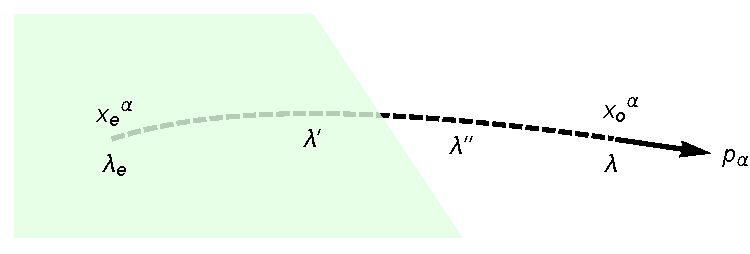
\includegraphics[width=\columnwidth]{fig-affine_parameter_label}
  \caption{Affine parameterization of a neutrino trajectory of momentum
    $p_\alpha$.
    The fiducial observer with velocity $u^\alpha$ sits at $x^\alpha_o$,
    the neutrino emission event is at $x^\alpha_e$. The affine parameter
    increases from the emission event: $\lambda_e<\lambda'<\lambda''$.}
  \label{fig:affine_param}
\end{figure}

\subsection{The Rendering Equation}
\label{ssec:rendering_eqn}
We can integrate Eqn.~\ref{eqn:boltzmann_split} directly, 
with our solution split into a boundary, absorption/emission, and
a scattering term, $f=f_{\rm bdry}+f_{\rm AE}+f_{\rm SE}$:
\begin{align}
  \label{eqn:rendering_fbdry}
  f_{\rm bdry}(\lambda,\lambda_e)
  &= f(\lambda_e) e^{-\tau(\lambda,\lambda_e)}, \\
  \label{eqn:rendering_fae}
  f_{\rm AE}(\lambda,\lambda_e)
  &= \int_{\lambda_e}^\lambda d\lambda'\,e^{-\tau(\lambda,\lambda')}
  \mathscr{K}_{\rm AE}(\lambda')f^{\rm eq}(\lambda'), \\
  \label{eqn:rendering_fse}
  f_{\rm SE}(\lambda,\lambda_e)
  &= \int_{\lambda_e}^\lambda d\lambda'\,e^{-\tau(\lambda,\lambda')}
  \mathscr{K}_{\rm SE}(\lambda')\Phi(\lambda'),
\end{align}
where the optical depth is defined,
\begin{equation}
  \label{eqn:optical_depth}
  \tau(\lambda,\lambda') \equiv -\int_{\lambda'}^\lambda
  d\lambda'' \, \mathscr{K}(\lambda''),
\end{equation}
and the parameterization conventions are depicted in
Fig.~\ref{fig:affine_param}.
Note that Eqn.~\ref{eqn:optical_depth} employs the total absorption
plus scattering opacity, so that the optical depth attenuating the
integrands of Eqns.~\ref{eqn:rendering_fae} and \ref{eqn:rendering_fse}
is the total optical depth.

%Note the following equivalents; we could use any of these to express
%the integrands above:
%\begin{align}
%  \mathscr{K}_{\rm AE} \, f^{\rm eq}
%  &= \mathscr{K}\, \mathscr{S}_{\rm AE}
%  = \mathscr{E}_{\rm AE},\nonumber \\
%  \mathscr{K}_{\rm SE} \, \Phi
%  &= \mathscr{K} \, \mathscr{S}_{\rm SE}
%  = \mathscr{E}_{\rm SE}.\nonumber
%\end{align}

\subsection{Moments of the Distribution Function}
\label{ssec:moments}
\todo{code these up}
We may take angular moments of the distribution function:
\begin{align}
  \label{eqn:J}
  J(\varepsilon) &=
  \frac{\varepsilon^3}{(2\pi)^3} \oint d\Omega' f(\varepsilon, \ell'_\beta) \\
  \label{eqn:Ha}
  H^\mu(\varepsilon) &=
  \frac{\varepsilon^3}{(2\pi)^3} \oint d\Omega' f(\varepsilon, \ell'_\beta) \ell'^\mu \\
  \label{eqn:Sab}
  S^{\mu\gamma}(\varepsilon) &=
  \frac{\varepsilon^3}{(2\pi)^3} \oint d\Omega' f(\varepsilon, \ell'_\beta) \ell'^\mu \ell'^\gamma,
\end{align}
representing specific energy density, specific energy flux, and
specific momentum flux, respectively.
Here ``specific'' refers to the quantity being integrable over neutrino energy.
\todo{relate moments to other frames?}
Integrals~\ref{eqn:J}--\ref{eqn:Sab} are performed over a solid angle in
momentum space while holding $\varepsilon$ constant:
$d\Omega \equiv d(\cos a)\,db$.
\todo{consistent with Eqn.~\ref{eqn:def_direction}?}
We will also make use of the number density and flux defined as
$G(\varepsilon)=J(\varepsilon)/\varepsilon$
and $K^\mu(\varepsilon)=H^\mu(\varepsilon)/\varepsilon$
respectively.

The energy-integrated moments are
\begin{equation}
  \label{eqn:J_H_S_eps_integrated}
  \big\{ J,H^\mu,S^{\mu\nu} \big\} = \int_0^\infty d\varepsilon \,
  \big\{ J(\varepsilon),H^\mu(\varepsilon),S^{\mu\nu}(\varepsilon) \big\},
\end{equation}
having dimension ${\rm energy}\,{\rm length}^{-3}$.

There are two sensible observers to use to define the frame in which these
moments are computed, that is defining the four-velocity of
Eqn.~\ref{eqn:def_momentum}:
a stationary (also called an Eulerian) observer,
and a fluid (also called a comoving) observer \cite{smar1980-gr_hydro}.
Definitions are given in App.~\ref{sec:def_momentum}.
We distinguish moments computed assuming an Eulerian observer with a tilde,
e.g. $\tilde{J}$, $\tilde{H}^\mu$, $\tilde{S}^{\mu\nu}$.
Note that these three Eulerian moments are identical to the lab-frame moments
$E$, $F^\mu$, and $P^{\mu\nu}$
defined in
\cite{shib2011-truncated_moment, ocon2015-gr1d_with_nu, fouc2015-m1_nsbh}.

\subsection{Numerical Implementation}
\label{ssec:numerical}
Much of our numerical implementation is borrowed from the geodesic evolution
system described in~\cite{bohn2016-code}.
We integrate Eqns.~\ref{eqn:geodesic_x} and~\ref{eqn:geodesic_p} in the form
given by \citep{hugh1994-eh_finding},
and Eqns.~\ref{eqn:rendering_fae}, \ref{eqn:rendering_fse},
and \ref{eqn:optical_depth} in the form given below.
By using the time-component of Eqn.~\ref{eqn:geodesic_x} ($dt=d\lambda \, p^t$)
we may transform our integrations to coordinate time.
The coupled system of ordinary differential equations is
\begin{align}
  \label{eqn:num_x}
  \frac{dx^i}{dt} &=
  g^{ij} \frac{p_j}{p^t} - \beta^{i},\\
  \label{eqn:num_p}
  \frac{dp_i}{dt} &=
  -\alpha \alpha_{,i} p^t
  + \beta^k_{,i} p_k
  - \frac{1}{2} g^{jk}_{,i}\frac{p_j p_k}{p^t},\\
  \label{eqn:num_tau}
  \frac{d\tau}{dt} &=
  - \frac{1}{p^t}\mathscr{K},\\
  \label{eqn:num_fae}
  \frac{df_{\rm AE}}{dt} &=
  \frac{1}{p^t}e^{-\tau}\mathscr{K_{\rm AE}} \,f^{\rm eq},\\
  \label{eqn:num_fse}
  \frac{df_{\rm SE}}{dt} &=
  \frac{1}{p^t}e^{-\tau}\mathscr{K_{\rm SE}} \,\Phi.
\end{align}

We integrate each ray until we reach a terminal optical depth of
$\tau_{\rm term}$ at the earliest effective emission event $x_e^\alpha$.
The concept of earliest emission event is a facetious construct we use
to allow us to truncate our integration at an event along the ray where any
further additions to the field are negligible due to the large optical depth
between $x_e^\alpha$ and $x_o^\alpha$.
We choose $\tau_{\rm term}=14$ so that $e^{-\tau_{\rm term}}<10^{-6}$,
and we then discard the contribution of $f_{\rm bdry}$
(Eqn.~\ref{eqn:rendering_fbdry}).

Since we don't know the emission event a priori,
we follow the integration backwards in time,
from $t_o$ to $t_e$.
We begin each integration by setting initial values for the variables at $t_o$.
The observer specifies $x^i_o$ and $p_{i,o}$,
and we set $f_{{\rm AE},o}=f_{{\rm SE},o}=0$ and $\tau_o=0$.

We integrate Eqns.~\ref{eqn:num_x}--\ref{eqn:num_tau} with adaptive step sizes,
using the 5th-order Dormand-Prince algorithm \cite{pres2007-nr_3rd_ed},
which produces an error estimate by comparing the 4th and 5th order solutions.
\todo{update to 3rd order Runge-Kutta}
After each step is taken, the errors for each of the 9 variables of
Eqns.~\ref{eqn:num_x}--\ref{eqn:num_tau} are compared.
If the maximum of these errors exceeds some absolute or relative threshold
\todo{specify ScaledAbsRel algorithm}
the step size is decreased and the step recomputed,
if it is below some threshold the next step size is increased.
% see OdeIntegrators::AdaptiveDense
% and OdeSteppers::DormandPrince5
% and OdeControllers::ProportionalIntegral_Base::StepSizeToAttempt
% and OdeErrorMeasures::ScaledAbsRel
\todo{specify}

The volume data are components of the metric $\psi_{\alpha\beta}$,
its derivatives $\psi_{\alpha\beta,\gamma}$,
and the hydrodynamical data $W$, $u_i$, $\varrho$, $T$, and $Y_e$.
These fields are stored in spectral representation.
If they are computed via hydrodynamical simulation, they are saved to disk
at specified coordinate times and interpolated
with spectral interpolation in space,
and 1st-order polynomial interpolation in time
(as described in \cite[App.~B]{bohn2016-code}).
If computed from a quasi-stationary solution to the
\todo{clarify quasistationary timescale}
general relativistic hydrodynamics equations,
a single time is stored to disk, and no time interpolation is needed.

\section{Code Tests}
\label{sec:tests}

To test our algorithm, we integrate the ray tracing equations
(Eqns.~\ref{eqn:num_x}--\ref{eqn:num_tau}) at one observation position
in the following configurations. This suite of configurations
may be understood as a hierarchy of increasing physical realism:
beginning with a homogeneous medium of effectively
infinite extent (i.e.\ optically thick) and progressing to a model of a
1D pre-supernova, post-bounce collapse profile
evolved using an M1 transport hydrodynamical simulation.
In the pre-supernova model, we compare ray tracing distributions
to those calculated in a Monte Carlo transport simulation.
Finally, we calculate global measures of the neutrino fields outside of the
hypermassive neutron star and disk formed in a binary neutron star
merger simulated by \cite{fouc2016-m1_nsns, fouc2016-m1_evolve_n},
and compare ray tracing results to those from the M1 transport simulation.

In the following we present two forms of the integrated distribution functions,
Eqns.~\ref{eqn:num_fae} and \ref{eqn:num_fse}:
1) the full form  by which the solution is $f_{\rm scat}=f_{\rm AE}+f_{\rm SE}$
(labeled `scat' since we include elastic scattering), and
2) the form treating only absorption/emission interactions
in which we set $\mathscr{K}_{\rm SE}=0$ so that $f_{\rm noscat}=f_{\rm AE}$
(labeled `no scat' since we ignore elastic scattering).
There is no simple relation between the two forms for a given ray; that is
$f_{\rm scat} \neq f_{\rm noscat}+f_{\rm SE}$.
This is because $f_{\rm AE}$ is integrated using solely the absorption optical
depth in the first form,
and the absorption plus scattering optical depth in the second form.
The differences between these two methods is apparent
in Fig.~\ref{fig:cumulative_f_homogeneous}.
Before this work, the noscat form of the equations has been the standard for
ray tracing, though many authors include the scattering optical depth in
the integration of Eqn.~\ref{eqn:num_fae}
(see for example \cite{hari2010-gr_nunubar_collapsar}).
\todo{explain why; cite others}

\subsection{Infinite Homogeneous Slab:
  Testing Thermodynamic Equilibrium}
\label{ssec:test_equilibrium}
In an optically thick region the radiation field is in thermodynamic equilibrium
with the matter.
We set up a large slab of matter
representative of the fluid in the Massive Collapsed Star test
(Sec.~\ref{ssec:test_collapse}) at the radius 50~km.
For comparision with that test we use the LS180 equation of state
\cite{latt1991-nuc_eos}
\footnote{available at \lstinline{stellarcollapse.org}}
in which the equilibrium $\nu_e$ neutrino chemical potential is
$\mu_{\nu_e}=-0.575$~MeV
(with $\mu_{\bar{\nu}_e}=-\mu_{\nu_e}$ and $\mu_{\nu_x}=0$).
Fig.~\ref{fig:mfps-50km} presents the neutrino mean free paths
at this thermodynamic point over two energy decades.
For this test we set up our slab large enough for neutrinos of all
energies to be trapped. 
Since our ray tracing algorithm integrates rays to terminal optical
depths of $\tau_{\rm term}>14$, our domain must extend to $r=10^7\,{\rm km}$.

Fig.~\ref{fig:cumulative_f_homogeneous} displays the integrated $f$ as a
function of path length along the ray.

Fig.~\ref{fig:homogeneous_isotropic} shows the error in our results.
\todo{describe with scat on}

\begin{figure}
  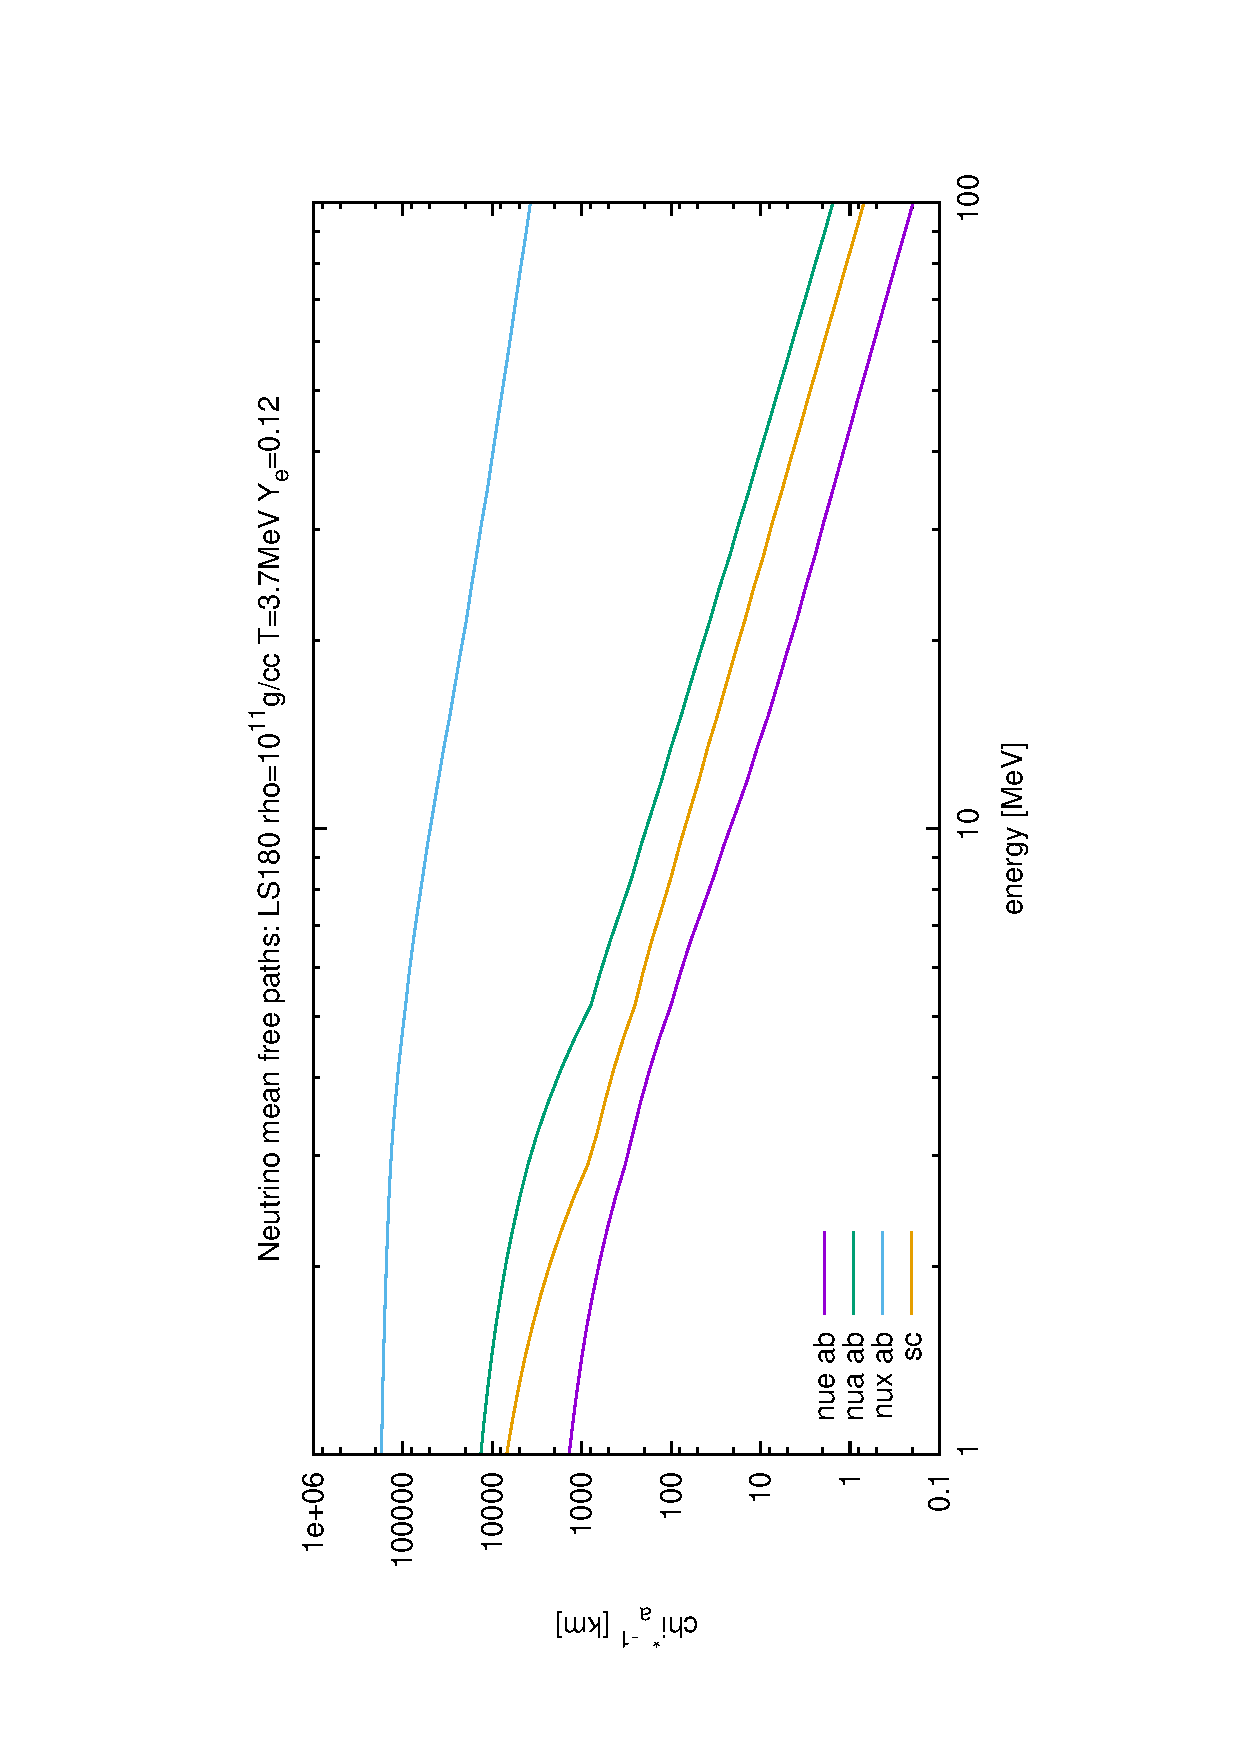
\includegraphics[width=\columnwidth]{figure-mfps-50km}
  \caption{Mean free paths
    representative of the collapse profile at
    50~km ($\varrho=10^{11}\,{\rm g}\,{\rm cm}^{-3}$,
    $T=3.7$~MeV, $Y_e=0.12$).
    In the fluid rest frame these are given by
    $(\chi^*_a)^{-1}$ for the absorption
    and $(\chi_s)^{-1}$ for elastic scattering interactions.
    Computed using \lstinline{NuLib}, as in the ray tracing code.
  }
  \label{fig:mfps-50km}
\end{figure}

\begin{figure}
  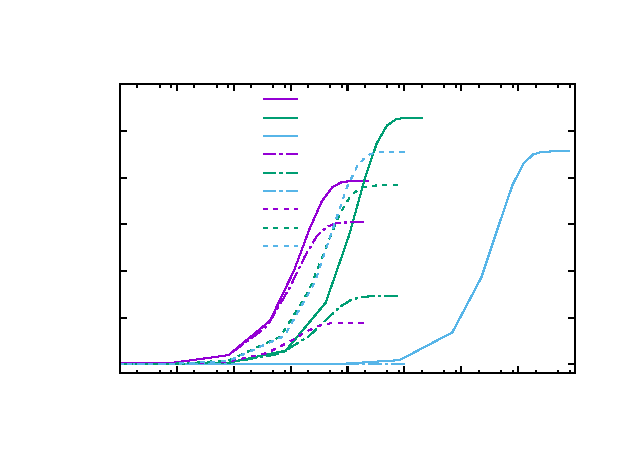
\includegraphics[width=\columnwidth]{fig-cumulative_f-homogeneous}
  \caption{Cumulative distribution functions at $\varepsilon=11.25$~MeV
    in homogeneous infinite slab of Sec.~\ref{ssec:test_equilibrium}.
    The integration proceeds from left to right (backwards in time $t$).
    The two components of the scat solutions ($f_{\rm AE}$ in points,
    and $f_{\rm SE}$ in dashed lines) sum to equal the single component
    of the noscat solution ($f_{\rm AE}$ in points connected by lines).
    All solutions terminate when they achieve a total optical depth
    greater than $\tau_term=14$; in the scat cases this occurs at an
    earlier time since the total mean free paths are less than the
    absorption mean free paths (much less in the case of $\nu_x$).
    The positions of the points (only plotted for the $f_{\rm AE}$ components)
    are the time steps chosen by the adaptive time-stepping algorithm
    described in Sec.~\ref{ssec:numerical}.
  }
  \label{fig:cumulative_f_homogeneous}
\end{figure}

\begin{figure}
  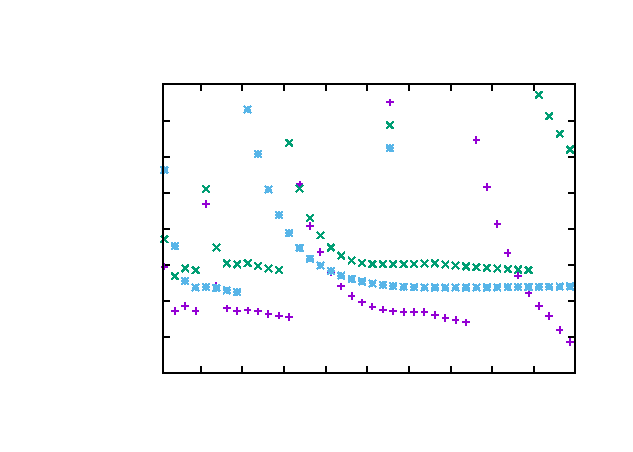
\includegraphics[width=\columnwidth]{figure-ferr-50km}
  \caption{Relative error in integrated equilibrium distribution functions
    in the infinite homogeneous slab  described in
    Sec.~\ref{ssec:test_equilibrium}.
    Presented here are the relative differences between the final
    $f_{\rm AE}$ in the noscat case
    (see Fig.~\ref{fig:cumulative_f_homogeneous})
    and the equilibrium distribution functions given by
    Eqn.~\ref{eqn:feq}.
    As can be seen in Fig.~\ref{fig:mfps-50km} these three species
    over the given energies
    probe our numerical solution over length scales from
    100~m to $10^{5}\,{\rm km}$.
    The source of this error is the discarded boundary term
    $f_{\rm bdry}\sim10^{-6}$, described in Sec.~\ref{ssec:numerical}.
  }
  \label{fig:homogeneous_isotropic}
\end{figure}

\subsection{Infinite Homogeneous Moving Slab:
  Testing Doppler Shift}
\label{ssec:test_doppler}
We reproduce the test above, but with the matter moving in
in the $+z$ direction, with the observer stationary.
Plot in Fig.~\ref{fig:avg_eps_doppler}.
\todo{redo test at same thermo point}
\todo{describe test}

\begin{figure}
  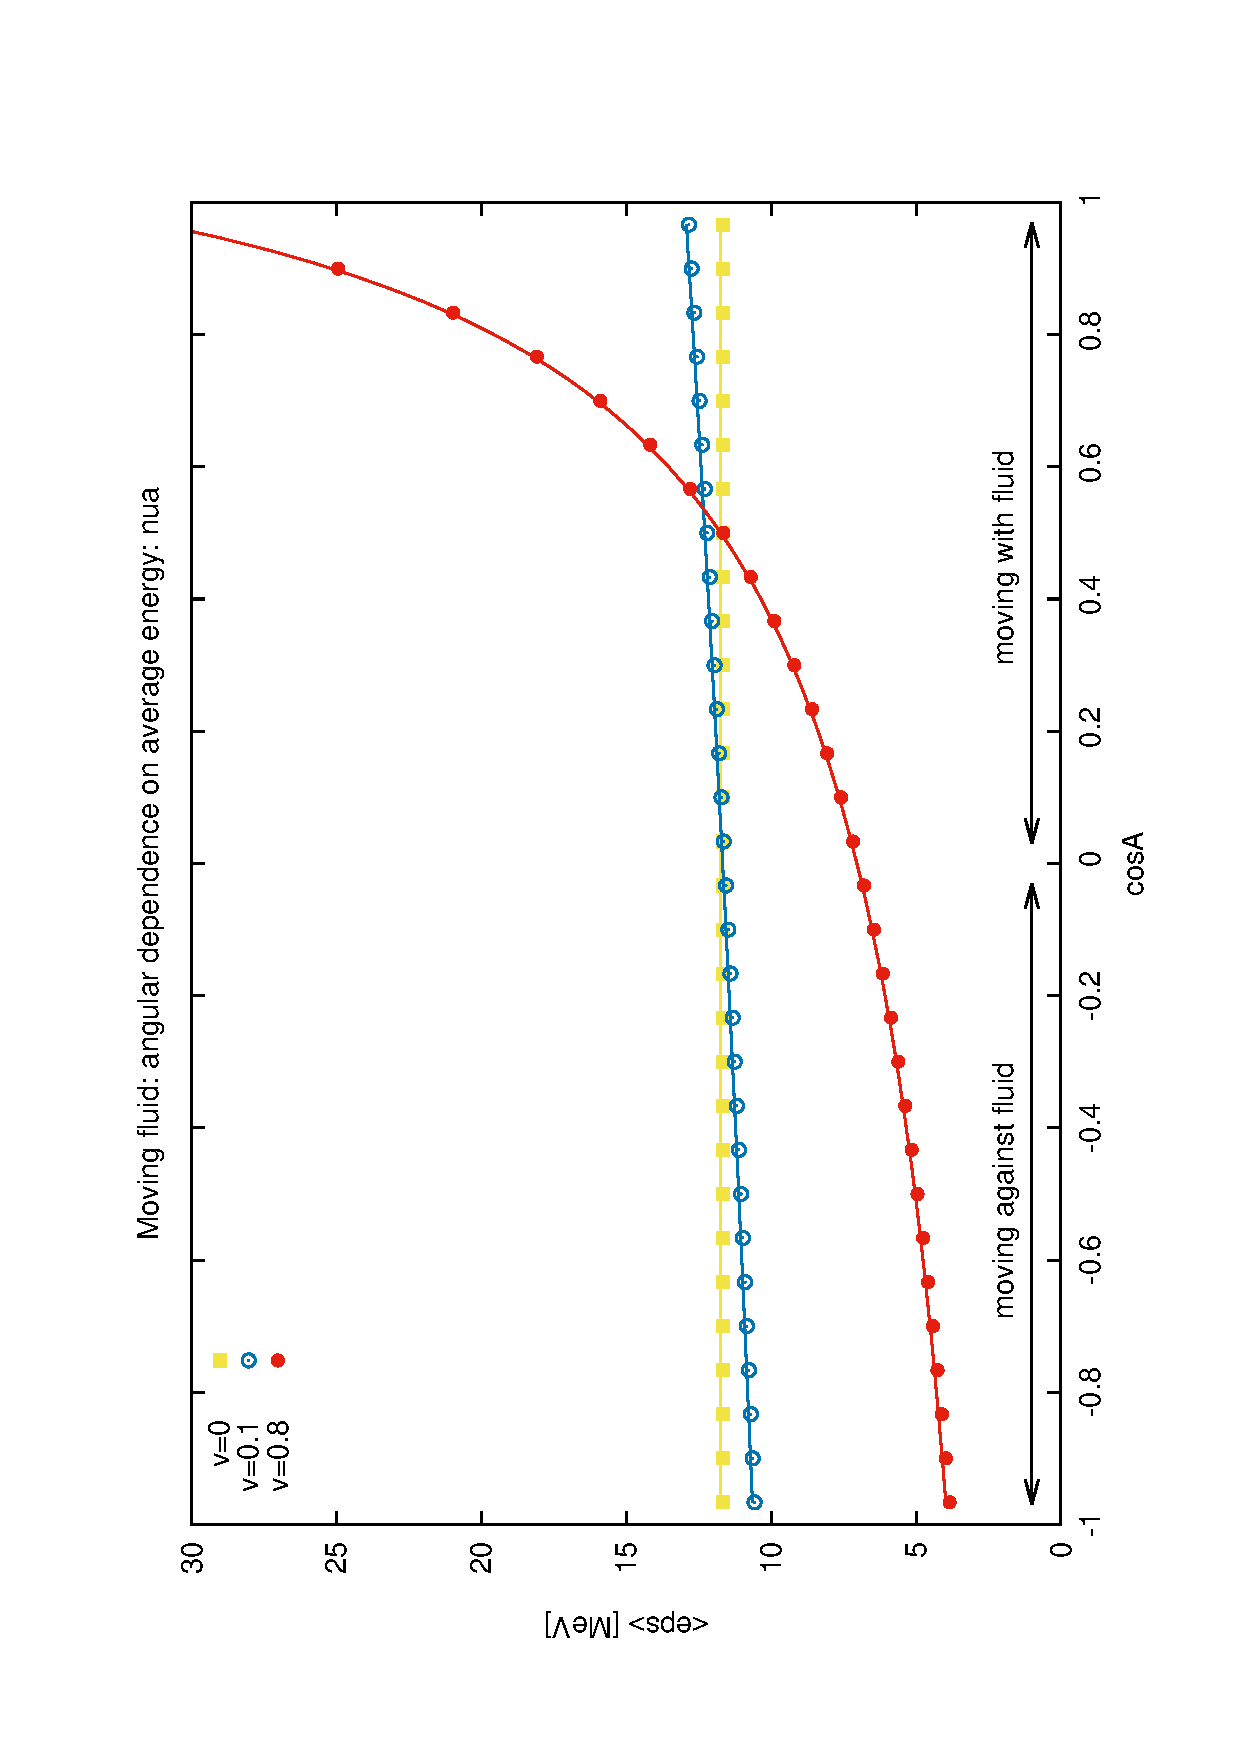
\includegraphics[width=\columnwidth]{fig-moving_fluid_avg_eps}
  \caption{Average energy $\langle\varepsilon\rangle(\cos A)=J(\cos A)/G(\cos A)$
    of $\bar{\nu}_e$ neutrino fields for fluid moving in the $+z$ direction,
    with $A$ the angle between the neutrino momentum and the $+z$ direction.
    Test described in Sec.~\ref{ssec:test_doppler}.
    The points are computed from ray tracing spectra; the lines are the
    analytic formula.
  }
  \label{fig:avg_eps_doppler}
\end{figure}

\subsection{Idealized Star:
  Testing the Decoupling Regime}
\label{ssec:test_ab_star}
[Test described in~\cite[Sec.~3.2]{smit1997-two_moment}.]
Plot in Fig.~\ref{fig:f_absorption_sphere}.

\begin{figure}
  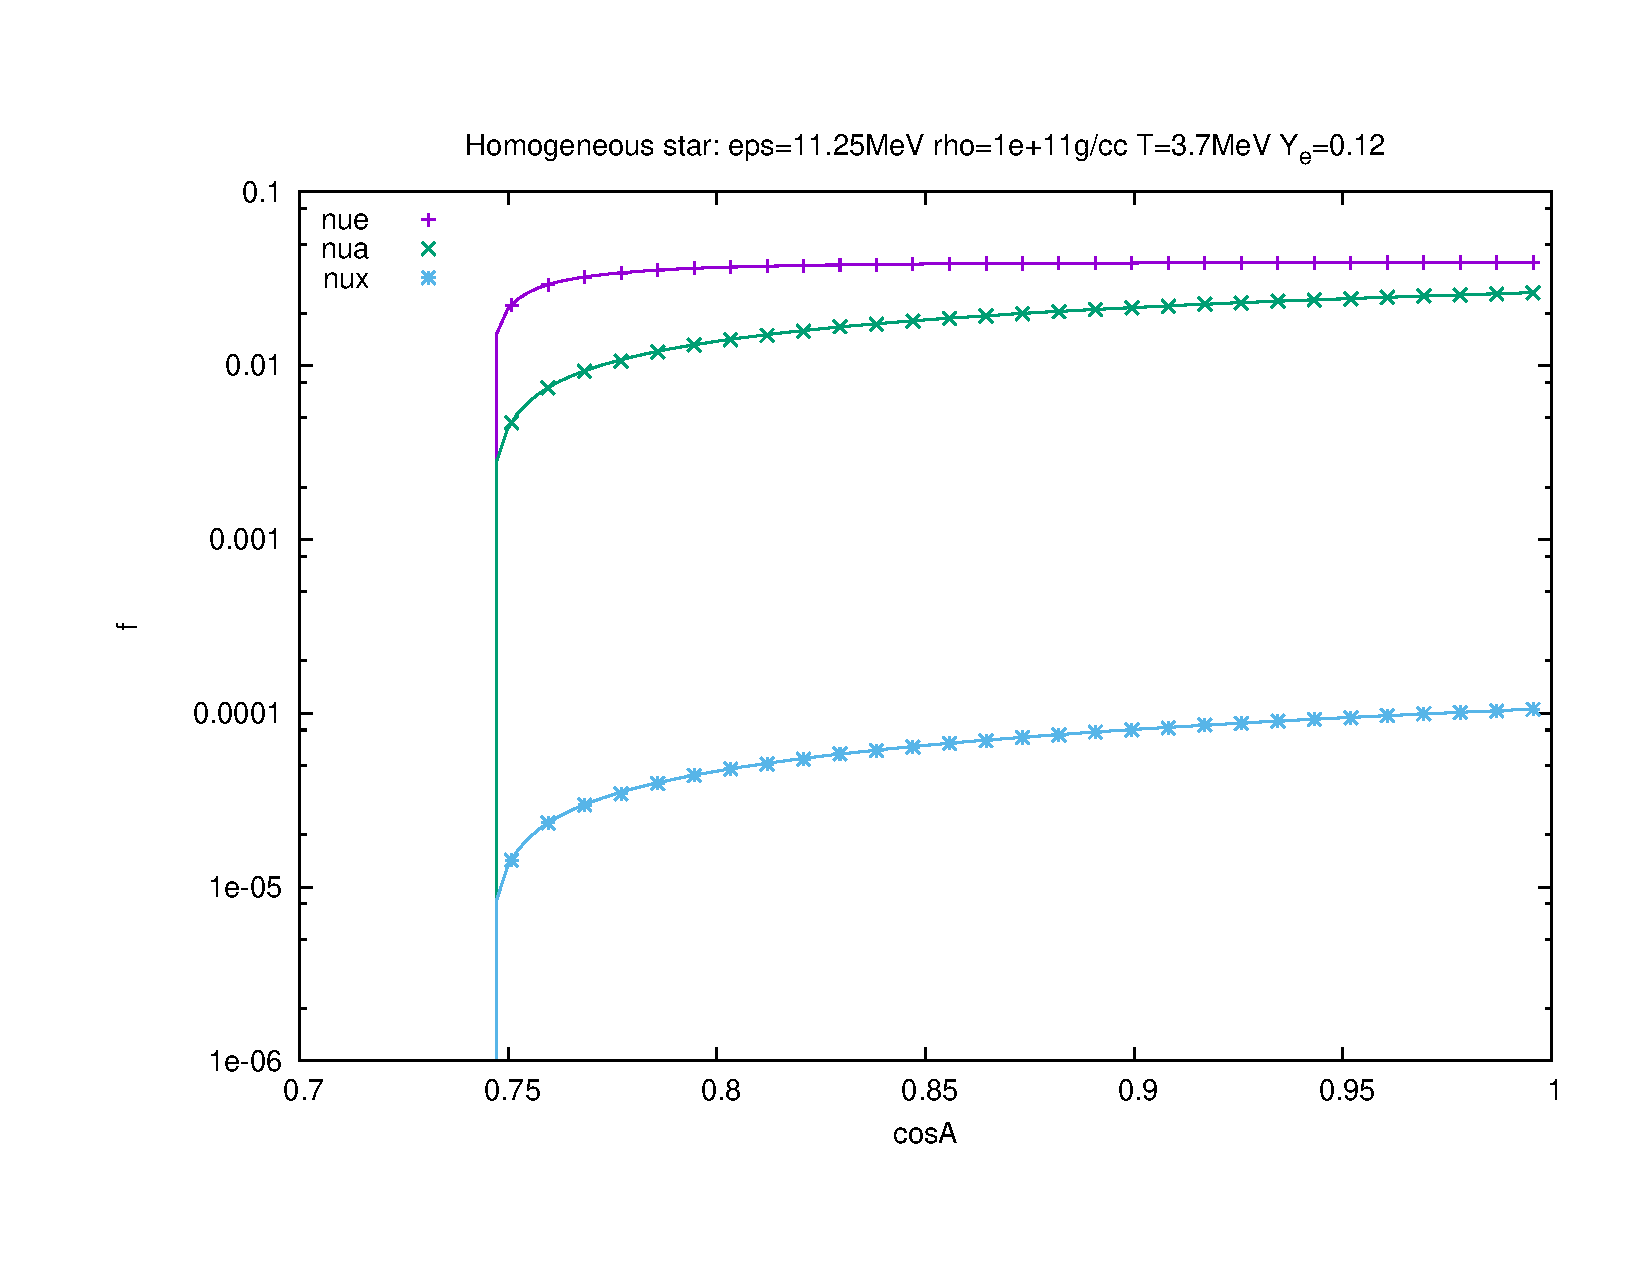
\includegraphics[width=\columnwidth]{fig-f-absorption_star-11MeV}
  \caption{Distribution functions outside an idealized homogeneous star
    with radius $R=50$~km, and observer at $r=75$~km.
    $A$ is the angle between the neutrino momentum and the $\hat{r}$ direction.
    The sample grid uses 40 points in energy linearly spaced across
    $\varepsilon\in(0,100)$~MeV,
    and 30 points in cosine of the polar angle linearly spaced across
    $\cos A\in(0.7377,1)$.
    To simplify this plot a single energy group only is displayed:
    $\varepsilon=11.25\,{\rm MeV}$.
    The points are computed from ray tracing; the lines from the analytic
    solution.
    Test described in Sec.~\ref{ssec:test_ab_star}.
  }
  \label{fig:f_absorption_sphere}
\end{figure}

\begin{figure}
  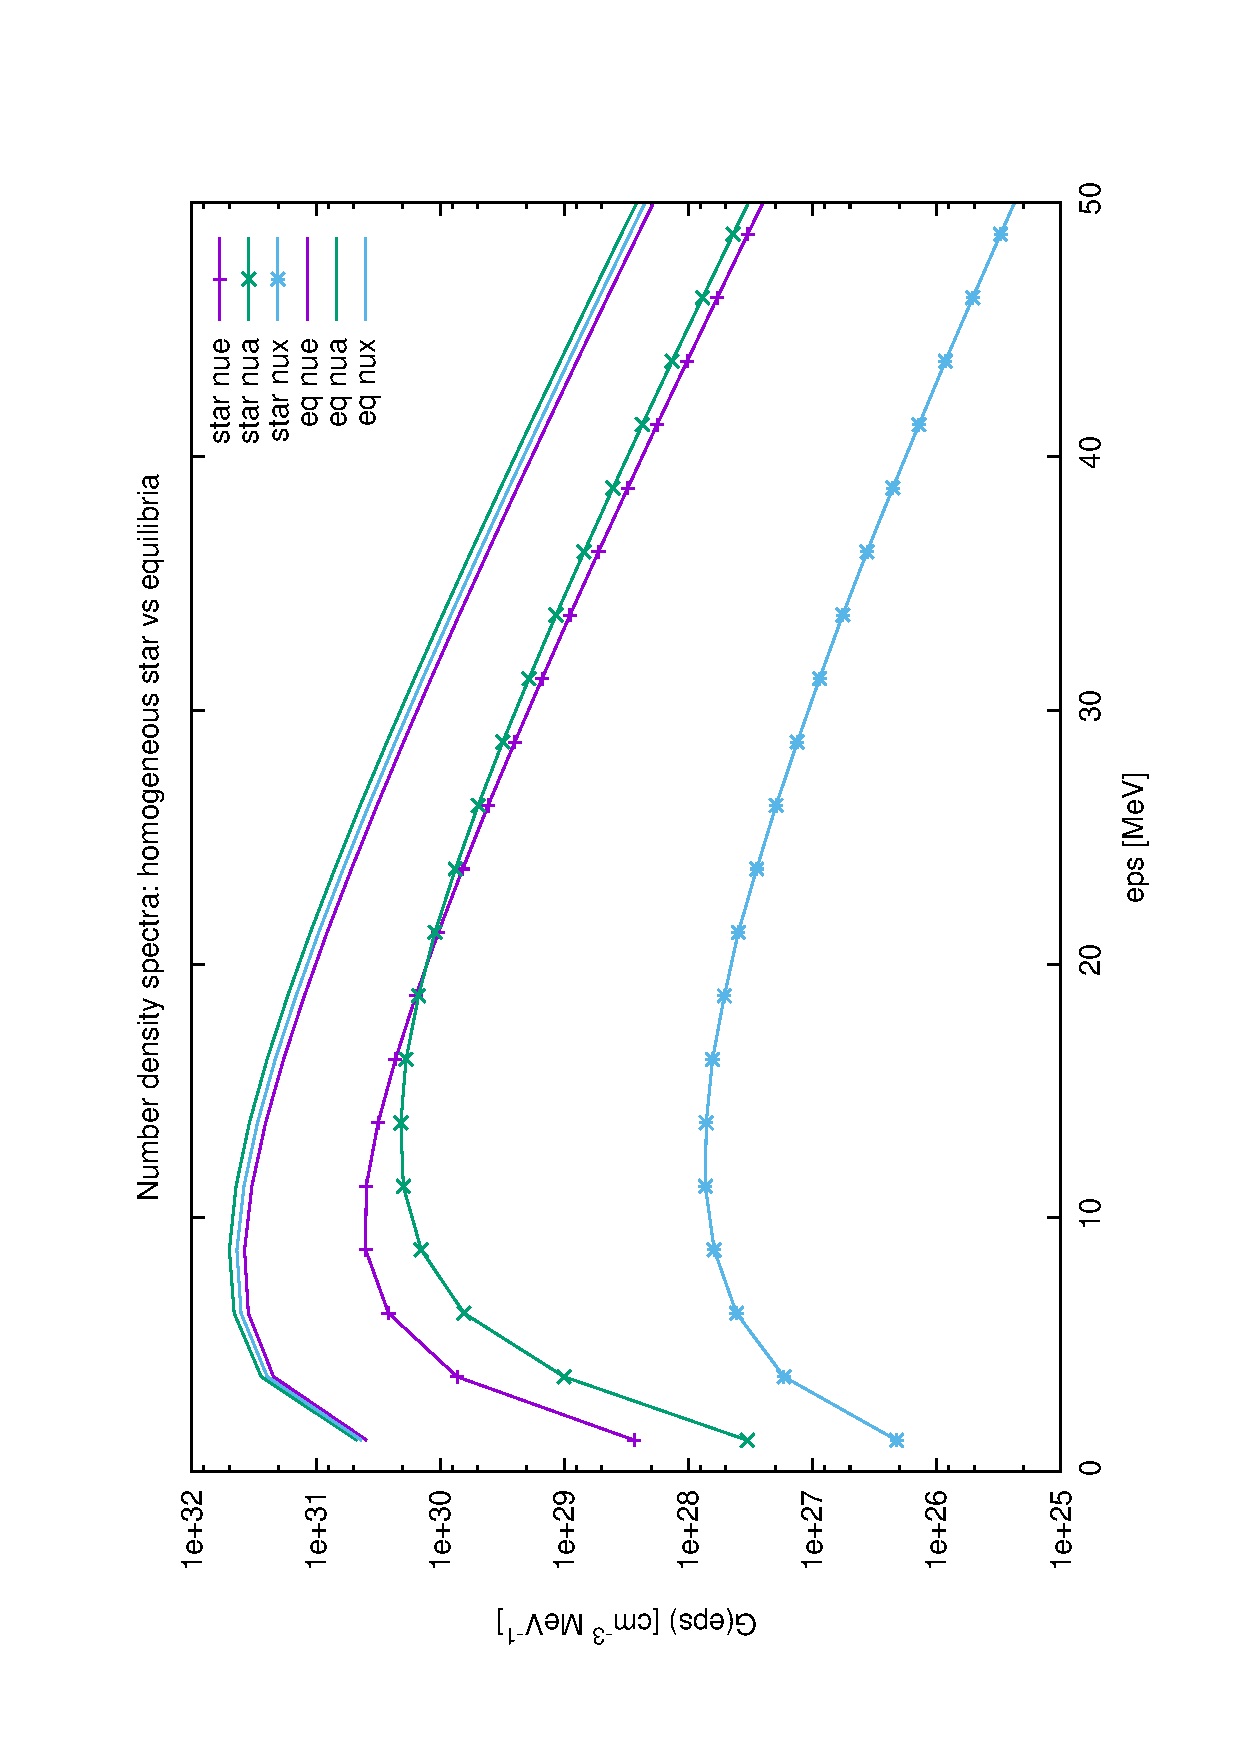
\includegraphics[width=\columnwidth]{fig-G_spectra-absorption_star}
  \caption{Number density spectra for an idealized homogeneous star.
    Test described in Sec.~\ref{ssec:test_ab_star}.
    The lines with points are the ray tracing spectra for this configuration;
    the solid lines are the ray tracincg spectra for an otherwise identical star
    of infinite extent (i.e. the spectra from Sec.~\ref{ssec:test_equilibrium}).
  }
  \label{fig:G_absorption_sphere}
\end{figure}

\subsection{Idealized Compact Star:
  Testing Gravitational Redshift and Geodesic Curvature}
\label{ssec:test_gravity}
Optically thick star in Schwarszchild.
Total luminosity at infinite separation may be computed by
computing the radial energy flux at a finite separation from the star, $r$,
and using $p_t$ for the energy. We compute this asymptotic luminosity
at several radii, $r$, and show that the luminosity is independent of
the observer's radius.
\todo{compute $L$, put in figure}

\subsection{Post-Bounce Collapse Profile:
  Testing Scattering}
\label{ssec:test_collapse}
[Standard radiation transport test described in~\cite{ocon2015-gr1d_with_nu},
and in \cite[App.~E.6]{fouc2015-m1_nsbh},
and in~\cite{abdi2012-monte_carlo}.]
\todo{clarify inelastic scattering and velocity terms}
Plot in Fig.~\ref{fig:avg_eps_collapse}.

\begin{figure}
  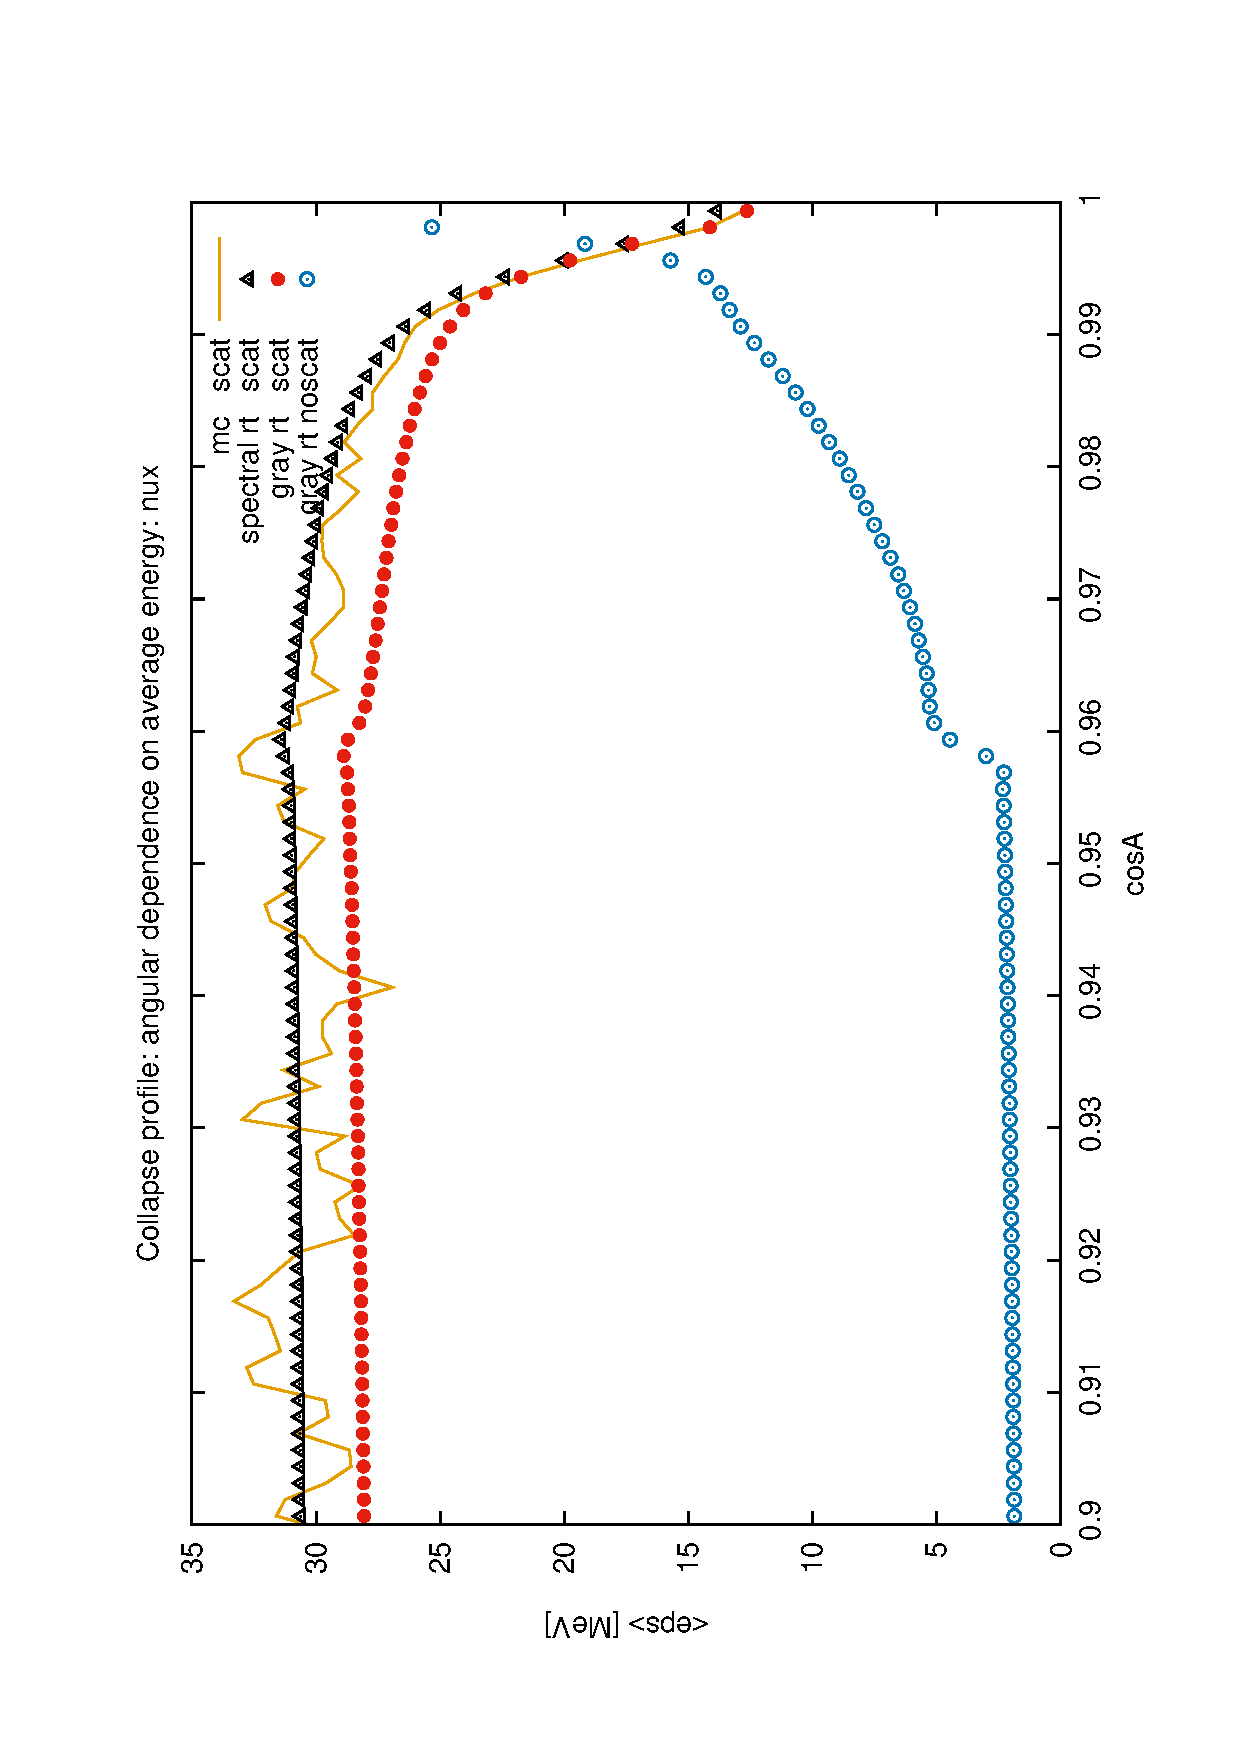
\includegraphics[width=\columnwidth]{fig-collapse_profile_avg_eps_vs_cosA}
  \caption{Average energies $\langle\varepsilon\rangle(\cos A)=J(\cos A)/G(\cos A)$
    in the collapse profile test described in Sec.~\ref{ssec:test_collapse}.
    The observer is at 500~km, and the shock at 150~km,
    so that the half-opening angle of the shock is $\cos A=0.954$.
    The four methods depicted are 1) a fiducial Monte Carlo calculation,
    ray tracing using the 2) spectral and 3) gray methods to estimate background
    fields for scattering, and 4) ray tracing neglecting scattering.
  }
  \label{fig:avg_eps_collapse}
\end{figure}

\subsection{Hypermassive Neutron Star Remnant:
  Testing Everything}
\label{ssec:test_disk_comparison}
The merger of two neutron stars by gravitational wave emission produces a
postmerger configuration composed of a single neutron star surrounded by a disk.
Because of the strong differential rotation of the remnant it temporarily avoids
collapse to a black hole, even if its mass exceeds the threshold of dynamical
instability for a rigidly rotating neutron star \cite{duez2009-review}.
These objects are called hypermassive neutron stars.

Such a configuration was modeled by \cite{fouc2016-m1_nsns} by
evolving the final inspiral and merger of two identical neutron stars of
isolated gravitational mass 1.2~$M_{\odot}$. The postmerger configuration
was evolved using an M1 transport scheme for the neutrinos, evolving the
energy density, number density, and energy flux \cite{fouc2016-m1_evolve_n}
for $\sim10\,{\rm ms}$ following merger, defined as the time of the peak of the
gravitational wave strain.

We used a single time snapshot of the volume data from that configuration
at $t=11\,{\rm ms}$ after merger (see
Figs.~\ref{fig:nsns_rho_merid}--\ref{fig:nsns_temp_equat})
sampling the neutrino fields with ray tracing to compare to some
measures of the field computed from the M1 transport simulation.

\begin{figure}
  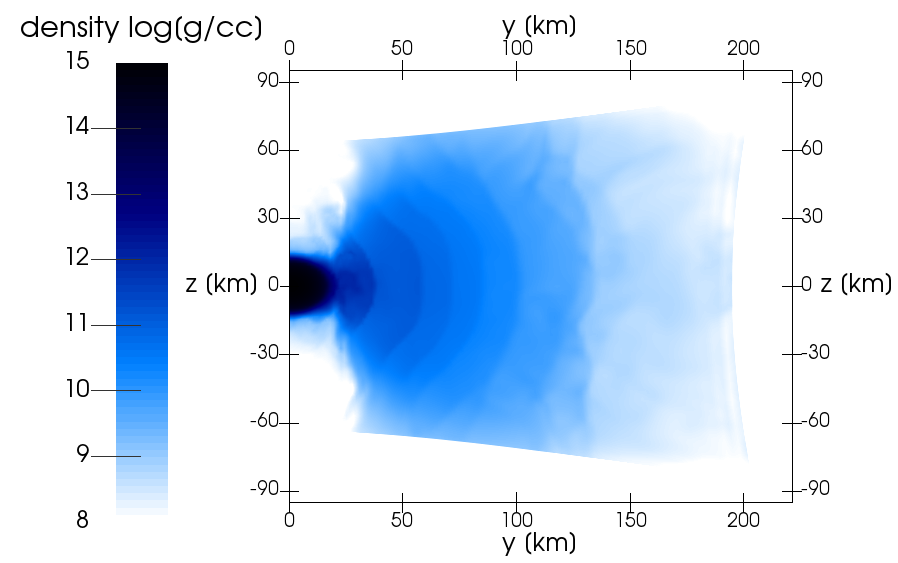
\includegraphics[width=\columnwidth]{production-colormap-merid-rho}
  \caption{A meridional slice of density in the hypermassive neutron
    star and disk configuration.
    The distorted rectangular boundaries are the boundaries of the grid
    used in the numerical simulation, which employs a coordinate mapping to
    concentrate points near the central object.}
  \label{fig:nsns_rho_merid}
\end{figure}

\begin{figure}
  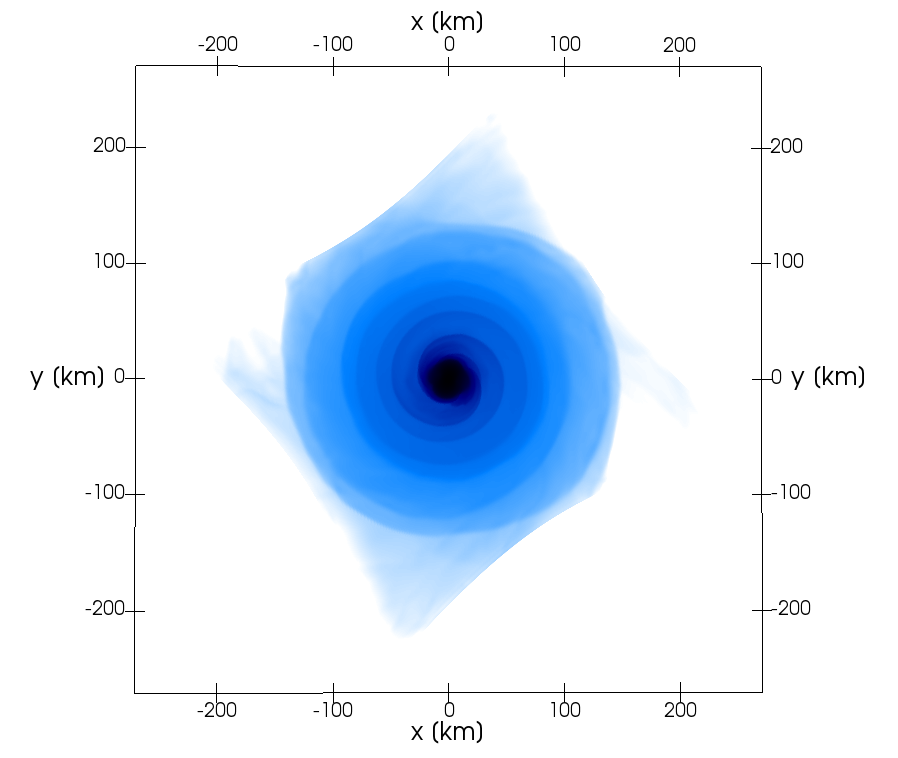
\includegraphics[width=\columnwidth]{production-colormap-equat-rho}
  \caption{An equatorial slice of density in the hypermassive neutron
    star and disk configuration.}
  \label{fig:nsns_rho_equat}
\end{figure}

\begin{figure}
  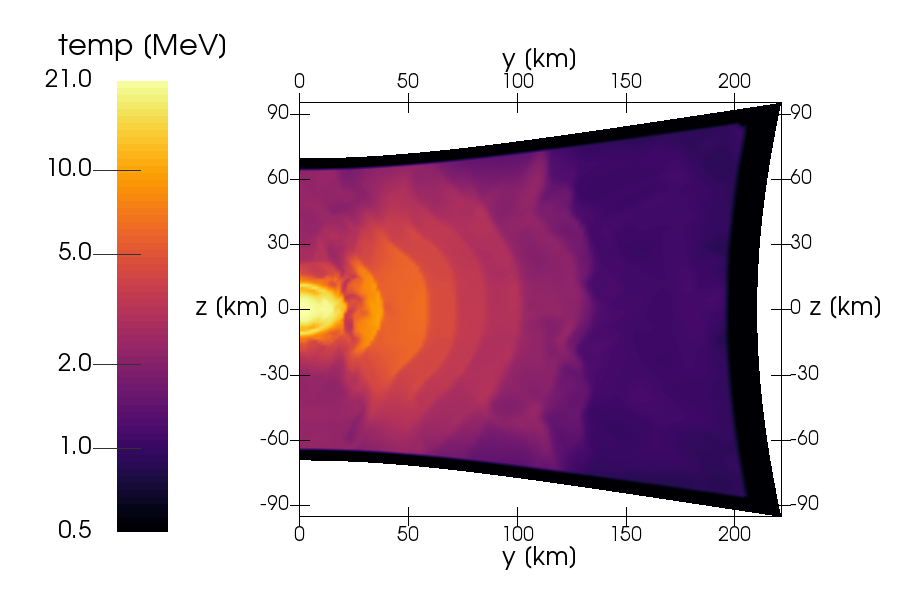
\includegraphics[width=\columnwidth]{production-colormap-merid-temp}
  \caption{A meridional slice of temperature in the hypermassive neutron
    star and disk configuration.}
  \label{fig:nsns_temp_merid}
\end{figure}

\begin{figure}
  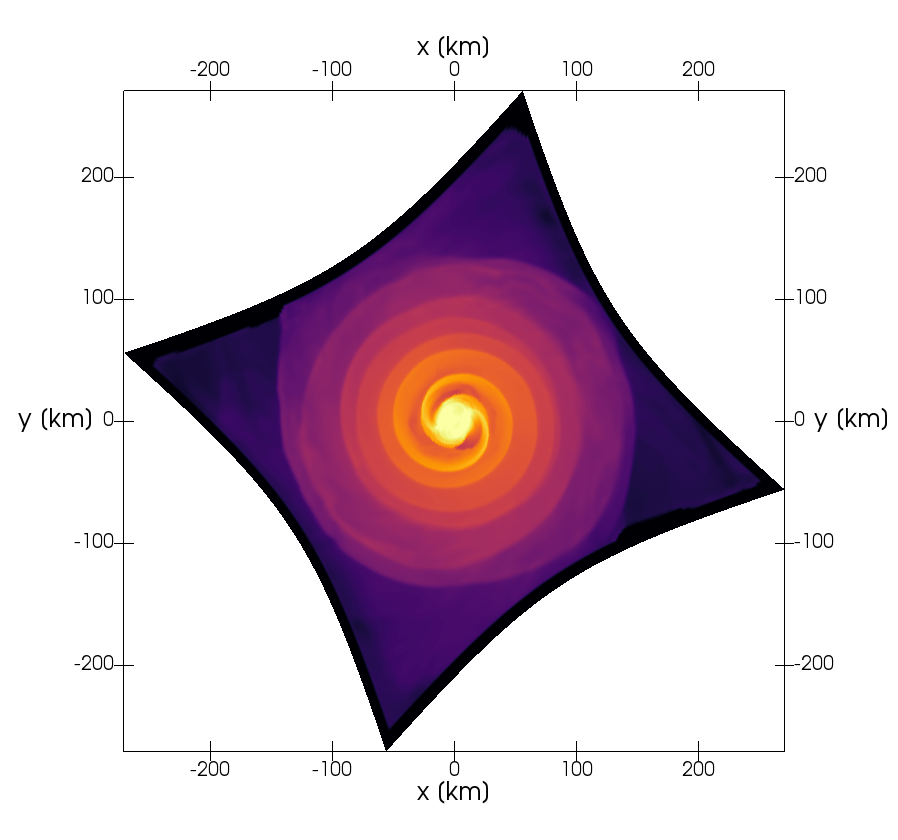
\includegraphics[width=\columnwidth]{production-colormap-equat-temp}
  \caption{An equatorial slice of temperature in the hypermassive neutron
    star and disk configuration.}
  \label{fig:nsns_temp_equat}
\end{figure}

In Tab.~\ref{tab:nsns_rt_vs_m1} we present total and relative number and
energy luminosities for this configuration.
With scattering turned off, ray tracing errors are as large as 250\%
(for heavy lepton energy luminosities).
But with scattering turned on, agreement is better than 20\%, and
in most cases much better.
\todo{get accurage M1 numbers from Francois}

\begin{table}%[h]
  \caption{
    Comparison of total luminosities and average energies between
    ray tracing and the M1 transport simulation.
    The ray tracing totals were computed from sums over
    observers placed in the $y$-$z$ plane along an arc at coordinate distance
    $r=250\,{\rm km}$ from the center of the star, at 30 positions
    distributed evenly in $\cos\theta$ over the colatitude range
    $\theta\in[0,90^{\circ}]$.
    M1 values are taken from \cite[Figs. 7, 9, 10]{fouc2016-m1_evolve_n}.
  }
  \label{tab:nsns_rt_vs_m1}
  \begin{tabularx}{\columnwidth}{X r r r}
    & \,\,{\bf RT noscat} & \,\,{\bf RT scat} & \,\,{\bf M1} \\
    \hline
    $L_{\nu_e}\,[10^{52}\,{\rm erg}\,{\rm s}^{-1}]$      & 5.95 & 6.01 & 5 \\
    $L_{\bar{\nu}_e}$                                    & 10.6 & 11.8 & 12 \\
    $L_{\nu_x}$                                          & 30.2 & 12.6 & 12 \\
    $R_{\nu_e}-R_{\bar{\nu}_e}\,[10^{57}\,{\rm s}^{-1}]$ & -1.06 & -1.86 & -2 \\
    $\langle \varepsilon_{\nu_e} \rangle\,[{\rm MeV}]$   & 12.08 & 11.88 & 12 \\
    $\langle \varepsilon_{\bar{\nu}_e} \rangle$          & 15.96 & 14.69 & 15 \\
    $\langle \varepsilon_{\nu_x} \rangle$                & 36.25 & 23.67 & 26 \\
    \hline
  \end{tabularx}
\end{table}

\section{Applications}
\label{sec:applications}

\subsection{Understanding Emission Spectra}
\label{ssec:spectra}
In this section, we use ray tracing's ability to track ``where the neutrinos
are coming from'' to understand the features in the emission distributions
presented in the code tests.

The merger models are described in \cite{fouc2015-m1_nsbh, fouc2016-m1_nsns}.
Something like this is presented in \cite[Figs.~10-11]{pere2014-nu_wind};
compare.

\begin{figure}
  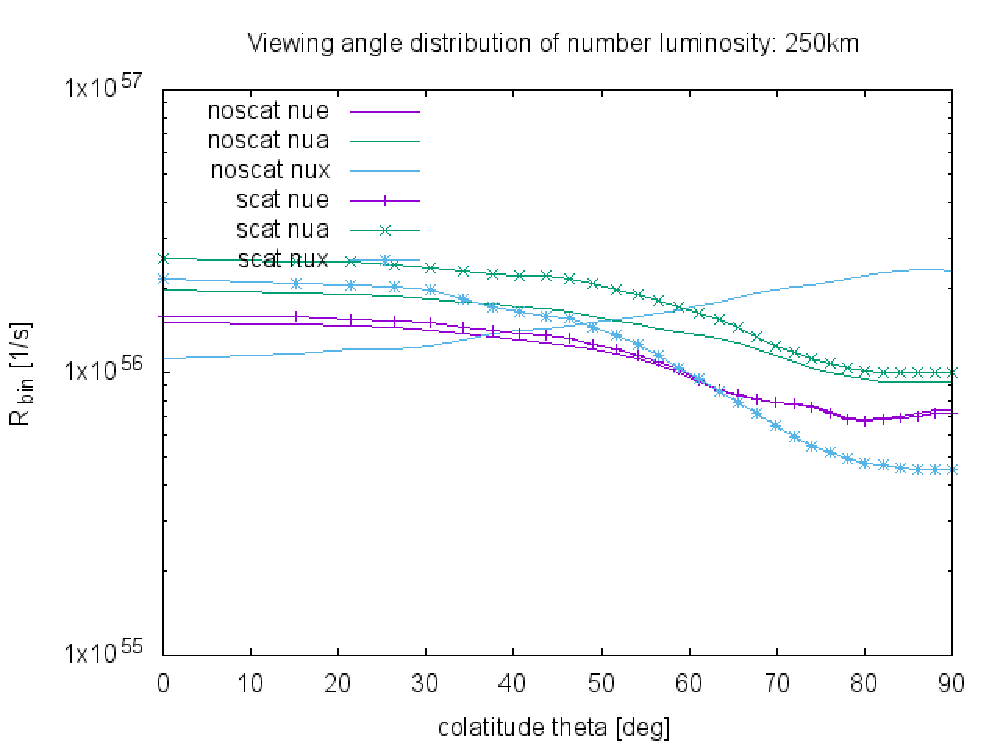
\includegraphics[width=\columnwidth]{theta_distrib-250km-luminosity_R}
  \caption{Radial number fluxes, $K_r$, as functions of colatitude $\theta$.
    Sampled for observers at fixed coordinate distances from the center
    of the star, with $r=250\,{\rm km}$.
    Here radial fluxes are multiplied by the portion of solid angle
    represented by each observer, so that the total luminosity is
    computed by summing all the points.}
  \label{fig:nsns_theta_distrib_R}
\end{figure}

\begin{figure}
  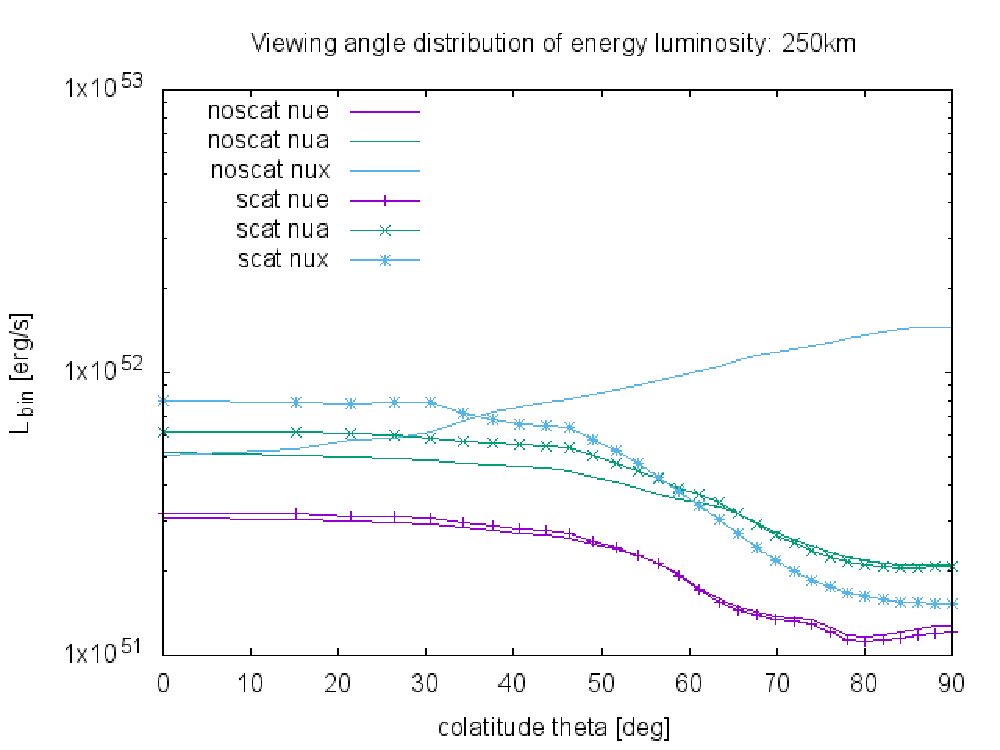
\includegraphics[width=\columnwidth]{theta_distrib-250km-luminosity_L}
  \caption{Same as Fig.~\ref{fig:nsns_theta_distrib_R} but radial energy
    fluxes, $H_r$.}
  \label{fig:nsns_theta_distrib_L}
\end{figure}

\begin{figure}
  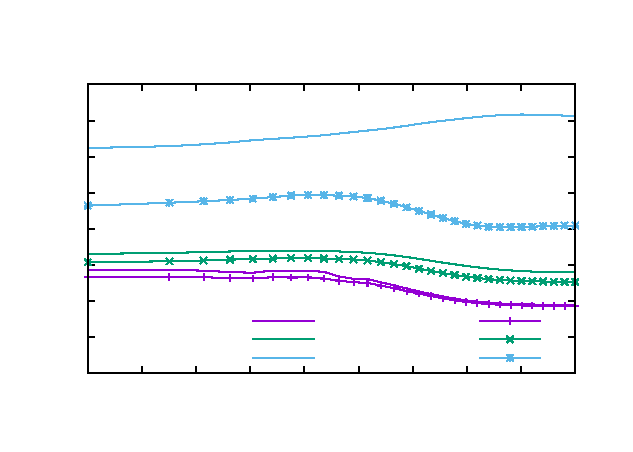
\includegraphics[width=\columnwidth]{theta_distrib-250km-avg_eps}
  \caption{Same as Fig.~\ref{fig:nsns_theta_distrib_R} but
    average energies $\langle \varepsilon \rangle = J/G$.}
  \label{fig:nsns_theta_distrib_avg_eps}
\end{figure}

\begin{figure}
  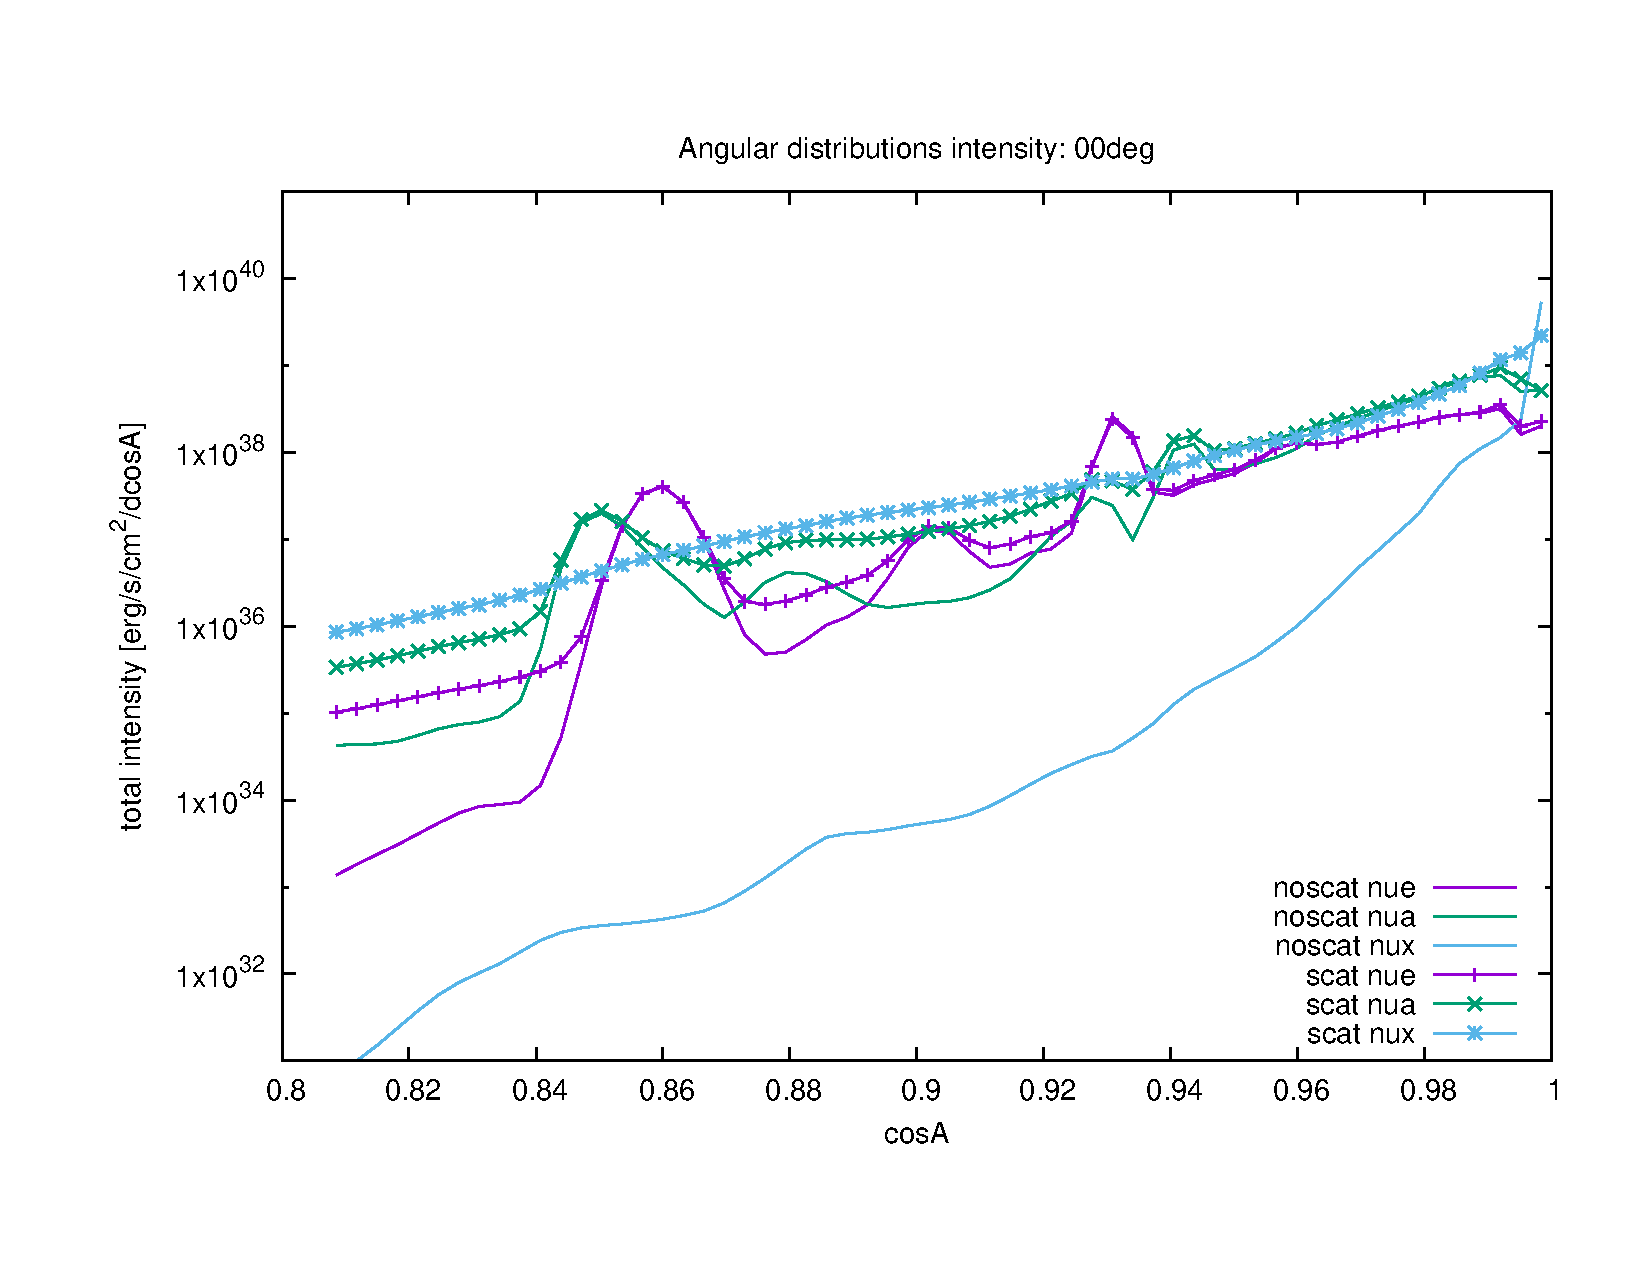
\includegraphics[width=\columnwidth]{cosA_distrib-intensity-250km-00deg}
  \caption{Angular distributions of fluxes for an observer on the rotation axis
    in the hypermassive neutron star configuration.}
  \label{fig:nsns_cosA_distrib_I_00deg}
\end{figure}

\begin{figure}
  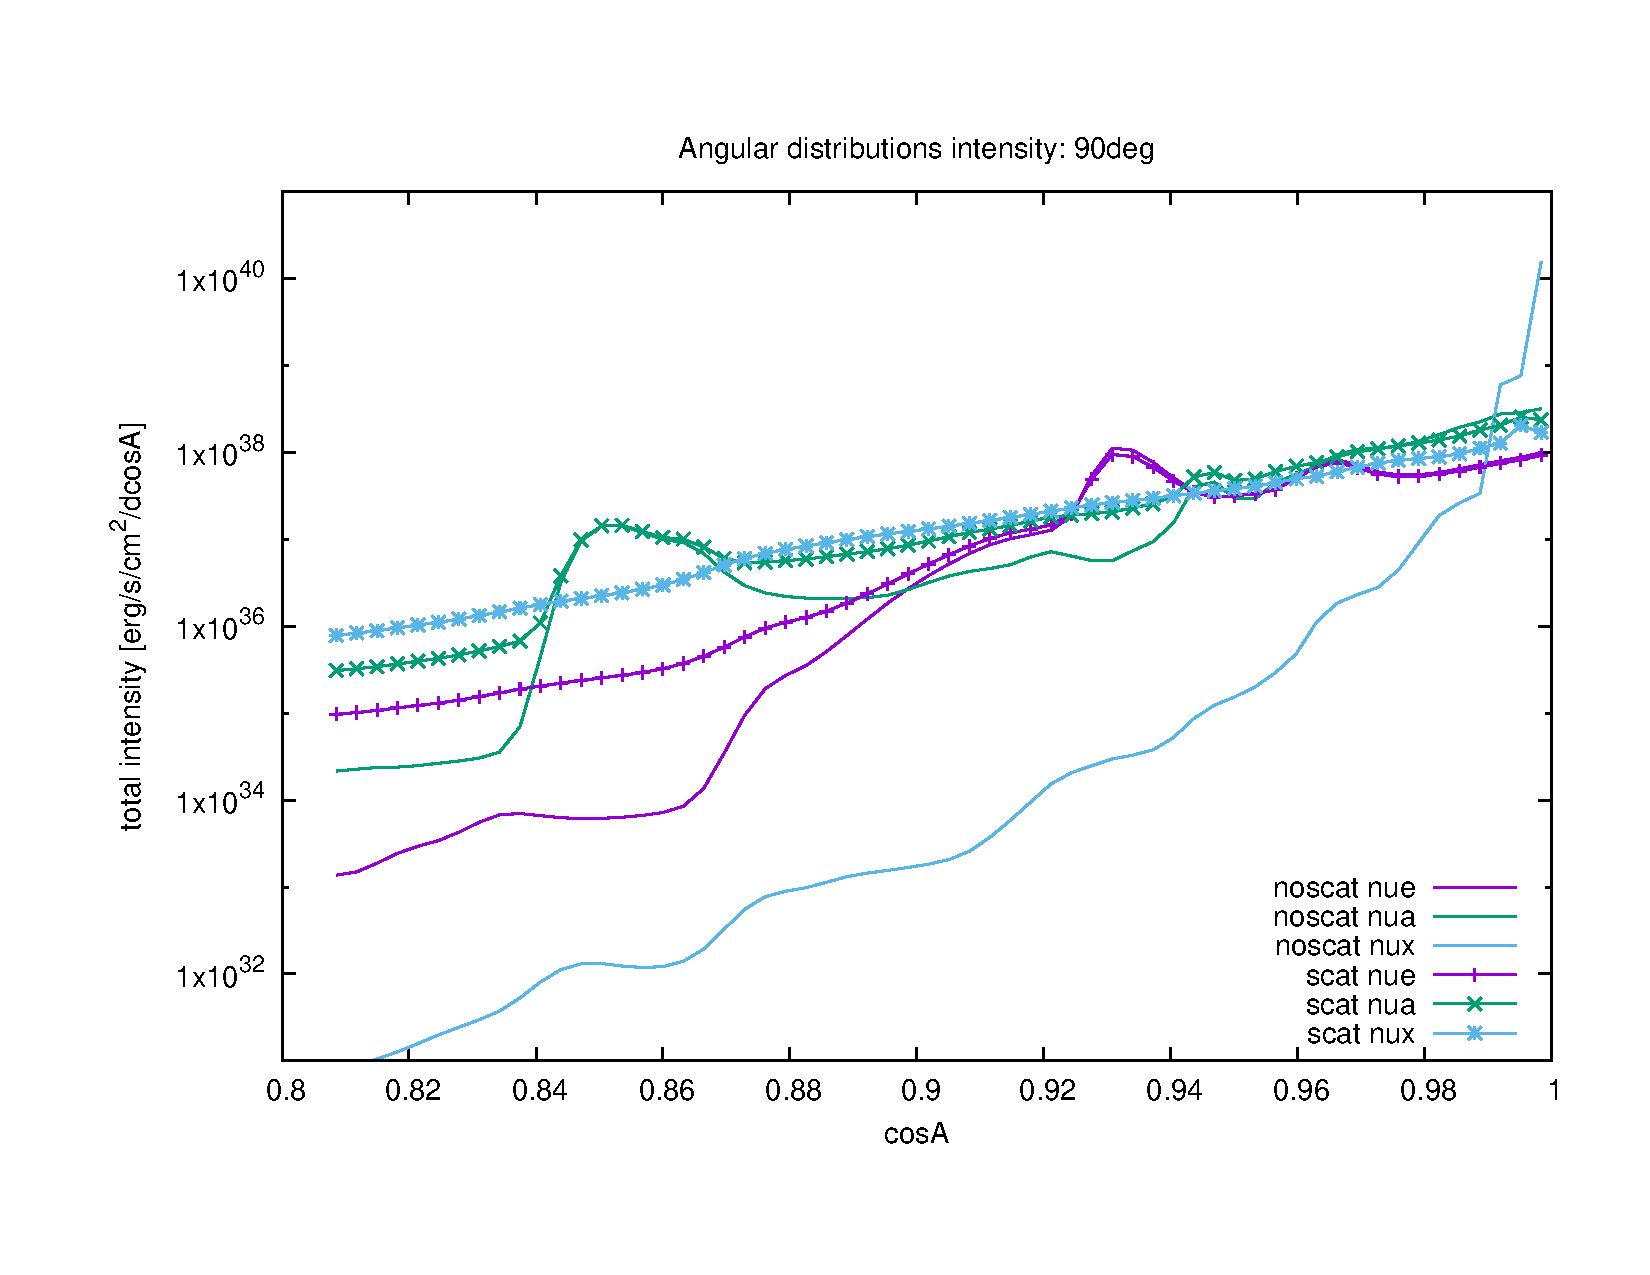
\includegraphics[width=\columnwidth]{cosA_distrib-intensity-250km-90deg}
  \caption{Angular distributions of fluxes for an observer in the equatorial
    plane in the hypermassive neutron star configuration.}
  \label{fig:nsns_cosA_distrib_I_90deg}
\end{figure}

\subsection{Neutrino Self-Interaction Potential}
\label{ssec:V_nunu}
In this section we present $V_{\nu\nu,0}$ along one test trajectory in the NSNS
model, and show that including elastic scattering makes a qualitative
difference in the character of the flavor evolution.
See Figs.~\ref{fig:V_nunu-noscat} and \ref{fig:V_nunu-scat}.

\begin{figure}
  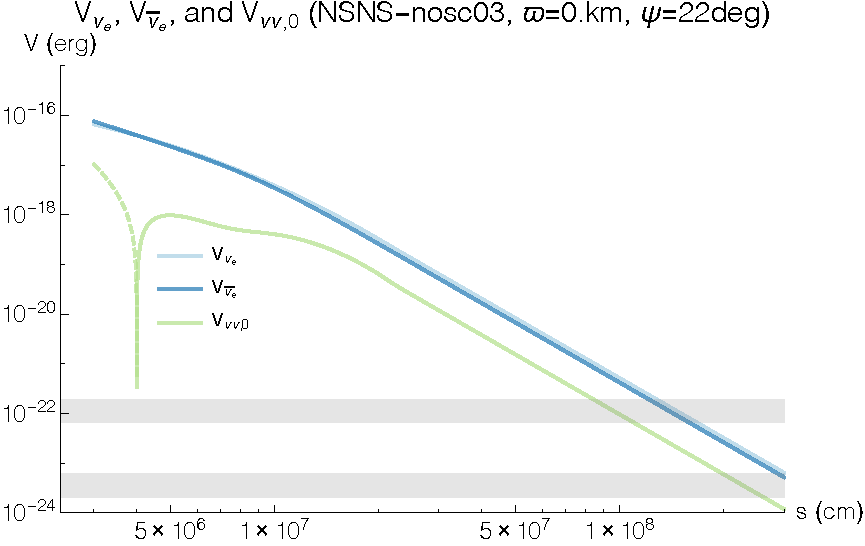
\includegraphics[width=\columnwidth]{20170619-potentials-Vnue_Vnua_Vnu-000Mo-022deg-noscat}
  \caption{Neutrino self-interaction potential along a test trajectory
    originating at the surface of the hypermassive neutron star, and
    proceeding outward along a radial coordinate ray with angle
    $\psi=22^{\circ}$ with respect to the polar axis.
    The trajectory is parameterized by the coordinate length $s$.
    This calculation was done with scattering turned off.
    Outside of the symmetric point at $s\sim40\,{\rm km}$, the potential is
    positive, i.e.\ $\nu_e$-dominated.
    Compare to Fig.~\ref{fig:V_nunu-scat}.
    }
  \label{fig:V_nunu-noscat}
\end{figure}

\begin{figure}
  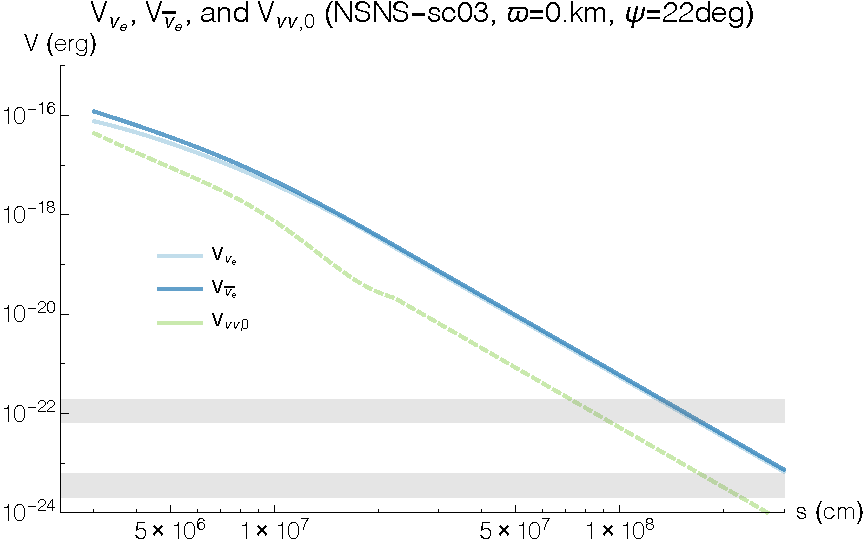
\includegraphics[width=\columnwidth]{20170619-potentials-Vnue_Vnua_Vnu-000Mo-022deg-scat}
  \caption{Same as Fig.~\ref{fig:V_nunu-noscat},
    but with scattering turned on.
    Unlike the case with scattering turned off, here the potential is
    everywhere negative, i.e.\ $\bar{\nu}_e$-dominated.
    }
  \label{fig:V_nunu-scat}
\end{figure}

\subsection{Neutrino Annihilation Integral}
\label{ssec:q_nunu}
In this section we calculate $q_{\nu\bar{\nu}}$ at a representative point
in the funnel of the NSNS configuration and show that including scattering makes
a difference (or not) in our estimate of the power available to drive a jet.

% ******************************************************************************
\appendix

\section{Momentum Definitions}
\label{sec:def_momentum}
Here we describe our conventions defining the four-momentum of a neutrino.
We decompose the neutrino momentum into components parallel and orthogonal to
an observer's velocity $u_\beta$:
\begin{equation}
  \label{eqn:def_momentum_2}
  p_\beta = \varepsilon (u_\beta + \ell_\beta),
\end{equation}
with $u_\alpha\ell^\alpha=0$ and $\ell_\alpha\ell^\alpha=1$.

In practice we use two possible fiducial observers to define the momentum
decomposition via Eqn.~\ref{eqn:def_momentum}: the Eulerian,
or normal observer $n_\mu=-\alpha \,\partial_\mu t$,
and the fluid, or comoving observer
$u^\mu=Wn^\mu+v_{\rm E}^\mu$.
Here $t$ is coordinate time and $\alpha$ is lapse
in the standard 3+1 decomposition of the metric
\begin{equation}
  \label{eqn:adm_metric}
  \psi_{\mu\gamma} \rightarrow
  \left(
  \begin{matrix}
    -\alpha^2 + \beta^i \beta_i  & \beta_i \\
    \beta_j                      & g_{ij}
  \end{matrix}
  \right).
\end{equation}
We have also introduced
the fluid Lorentz factor $W=-n_\mu u^\mu=\alpha u^t$,
its Eulerian velocity $v_{\rm E}^\mu=g^\mu_\lambda u^\lambda$
(distinct from its coordinate velocity $v^\mu=u^\mu/u^t$),
and the projection tensor orthogonal to the normal observer
$g^\mu_\lambda=\psi^\mu_\lambda+n^\mu n_\lambda$,
whose spatial part is the 3-metric, $g_{ij}$.

We specify the neutrino direction in the observer's frame
with two spherical polar angles
($a$,$b$) with respect to the simulation cartesian coordinates
\begin{align}
  \ell_\alpha &\rightarrow q(s,\Omega_i), \\
  \Omega_i &\rightarrow (\sin a \cos b,\sin a\sin b,\cos a),
\end{align}
or alternatively the two spherical polar angles
($A$,$B$) with respect to rotated coordinates
\begin{equation}
  \label{eqn:def_direction_primed_2}
  \Omega_{i'} \rightarrow  (\sin A \cos B,\sin A\sin B,\cos A).
\end{equation}
The two coordinate systems are related by a standard Euler rotation of first
$\phi$ about the $z$-axis, then $\theta$ about the rotated $y$-axis,
with $\phi$ and $\theta$ the azimuthal and polar position of the observer.
Expressed algebraically:
\begin{align}
  \label{eqn:rotation_connection}
  \Omega_x &= \Omega_{x'}\cos\theta\cos\phi-\Omega_{y'}\sin\phi+\Omega_{z'}\sin\theta\cos\phi,\nonumber\\
  \Omega_y &= \Omega_{x'}\cos\theta\sin\phi+\Omega_{y'}\cos\phi+\Omega_{z'}\sin\theta\sin\phi,\nonumber\\
  \Omega_z &= \Omega_{x'}\sin\theta+\Omega_{z'}\cos\theta.
\end{align}

The scale factors $q$ and $s$ are functions of the neutrino
direction $\Omega_i$, the observer's velocity $u_\alpha$,
and the spacetime metric.
In the case of a fluid observer, specified by an arbitrary $W$ and $u_i$,
$q$ and $s$ are given by
\begin{align}
  \label{eqn:q_general}
  q
  &= W\alpha\Bigg(2\beta^i\Omega_i W^2(\beta^i\Omega_i-1) \nonumber\\
  &\qquad\qquad - 2\Omega_i u_j g^{ij} W \alpha(\beta^i\Omega_i-1)\nonumber\\
  &\qquad\qquad + \alpha^2\left((\Omega_i u_j g^{ij})^2+\Omega_i\Omega_j g^{ij}W^2\right)\Bigg)^{-1/2}\\
  \label{eqn:s_general}
  s
  &= \beta^i\Omega_i -\Omega_i u_j g^{ij}.
\end{align}
In the case of an Eulerian observer, $W=1$ and $u_i=0$,
and these expressions simplify considerably:
\begin{align}
  \label{eqn:q_eulerian}
  \tilde{q}
  &= \alpha\left(2\beta^i\Omega_i(\beta^i\Omega_i-1)+\alpha^2\Omega_i\Omega_j g^{ij}\right)^{-1/2}\\
  \label{eqn:s_eulerian}
  \tilde{s}
  &= \beta^i\Omega_i.
\end{align}
In the even simpler case of Minkowski spacetime, these expressions
reduce to $q=W/(1+s)$, $s=-\Omega_i u^i$,
$\tilde{q}=1$, $\tilde{s}=0$.

\section{Source Terms}
\label{sec:source_terms}
Here we present the sources comprising the right hand side of the
Boltzmann Equation (Eqn.~\ref{eqn:boltzmann}). The sources for the neutrino
distribution function $f(x^\alpha;p_\beta)$ arise from collision processes
producing, removing, or scattering to/from that point in phase space.
The weak interaction rates for each process involve integrals of
the neutrino distribution function $f(x^\alpha;p'_\beta)$ and that of the
antineutrino $\bar{f}(x^\alpha;p'_\beta)$ over a momentum volume
$dP'$ (Eqn.~\ref{eqn:dP}).

We follow
\cite{brue1985-core_collapse} and \cite[Sec.~4]{shib2011-truncated_moment}
by separating these processes into four categories:
\begin{equation}
  \label{eqn:four_sources}
  C[f] \equiv C_{\rm AE} + C_{\rm SE} + C_{\rm SI} + C_{\rm PP},
\end{equation}
representing charged-current absorption and emission, elastic scattering,
inelastic scattering, and the thermal pair processes of annihilation and
production. In this work, however, we only treat absorption/emission
and elastic scattering.
We seek to write each collision source linear in $f$:
\begin{align}
  \label{eqn:sources_cae}
  C_{\rm AE}
  &= \mathscr{E}_{\rm AE} + \mathscr{K}_{\rm AE}\, f, \\
  \label{eqn:sources_cse}
  C_{\rm SE}
  &= \mathscr{E}_{\rm SE} + \mathscr{K}_{\rm SE}\, f.
\end{align}

Each term
is computed by summing the weak interaction rates of the processes from the
relevant category given in Tab.~\ref{tab:neutrino_processes}.
We compute these rates in the rest frame of the fluid,
but because they are spacetime invariants
they take the same numerical value in any frame of reference
and are completely independent of our choice of fiducial observer $u^\alpha$
(see discussion around Eqn.~\ref{eqn:boltzmann_linear}).

Each source term is unique to the neutrino or antineutrino species modeled,
and consists of a sum over all of the processes contributing to that
category of interaction. For example:
$C^{\nu_e}_{{\rm AE}} = \sum_i\,C^{\nu_e}_{{\rm AE},i}$,
where $i$ labels the absorption/emission processes involving $\nu_e$
in Tab.~\ref{tab:neutrino_processes}.
By contrast $C^{\nu_x}_{{\rm AE}} = 0$,
\todo{but we use a nonzero $C^{\nu_x}_{{\rm AE}}$}
where $\nu_x$ stands for any of the four heavy-lepton neutrinos and
antineutrinos.

We compute our rates using the open source neutrino interaction
library \lstinline{NuLib}~\footnote{\url{http://www.nulib.org}}.
We compile a table of sources defined over the four dimensions of
density, temperature, electron-fraction, and neutrino energy, and
interpolate quad-linearly to the points sampled along each ray.

\begin{table}%[h]
  \caption{
    We analyze neutrino interaction processes in terms of these categories.
    $\nu$ without a label represents a neutrino or antineutrino of any flavor,
    $N$ represents a nucleon $n$ or $p$,
    ${}^ZA$ represents a nucleus with mass number $A$ and charge $Z$, and
    $\gamma$ represents a high-energy photon.
    A prime indicates a change in that particle's energy.
  }
  \label{tab:neutrino_processes}
  \begin{tabularx}{\columnwidth}{X X}
    \hline \hline
    absorption/emission
    & $\nu_e + n \leftrightarrow e^- + p$                          \\
    & $\bar{\nu}_e + p \leftrightarrow e^+ + n$                    \\
    & $\nu_e + {}^AZ \leftrightarrow e^- + {}^A(Z+1)$              \\
    & $\bar{\nu}_e + {}^AZ \leftrightarrow e^+ + {}^A(Z-1)$        \\
    \hline
    elastic scattering
    & $\nu + N \leftrightarrow \nu + N$                            \\
    & $\nu + {}^AZ \leftrightarrow \nu + {}^AZ$                    \\
    \hline
    inelastic scattering
    & $\nu + e^- \leftrightarrow \nu' + e^{-'}$                    \\
    & $\nu + e^+ \leftrightarrow \nu' + e^{+'}$                    \\
    \hline
    thermal pair processes
    & $\nu + \bar{\nu} \leftrightarrow e^{-} + e^{+}$              \\
    & $\nu + \bar{\nu} + N + N \leftrightarrow N' + N'$            \\
    & $\nu + \bar{\nu} \leftrightarrow \gamma$                     \\
    % & $\nu_\alpha + \bar{\nu}_\alpha \leftrightarrow \nu_\beta + \bar{\nu}_\beta $ \\
    \hline \hline
  \end{tabularx}
\end{table}

\subsection{Absorption and emission via charged current}
\label{ssec:sources_ae}
At neutrino and thermal energies well below the masses of the muon or tauon
($m_{\mu}\sim100\,{\rm MeV}$)
only charged current processes involving $\nu_e$ and $\bar{\nu}_e$ are allowed.
For each of these processes, $i$, we may write an emission and absorption
coefficient as a function of the interaction cross-section
(e.g. \cite[Eqn.~A5]{brue1985-core_collapse}):
\todo{explain Fermi-blocking}
\begin{align}
  \label{eqn:sources_ae_1}
  C_{{\rm AE},i}
  &= \varepsilon j_i (1-f) - \varepsilon \chi_{a,i} f \\
  \label{eqn:sources_ae_2}
  &= \varepsilon j_i - (\varepsilon j_i+\varepsilon \chi_{a,i}) f,
\end{align}
where $j$ is the emissivity and $\chi_a$ the absorption opacity.
Both $j$ and $\chi_a$ have dimension ${\rm length}^{-1}$ and represent the
number of neutrinos emitted or absorbed per length traveled.
In radiation transport formulations using specific intensities instead of
distribution functions, an emissivity $\eta$ having dimension
${\rm energy}\,{\rm length}^{-3}\,{\rm time}^{-1}\,{\rm energy}^{-1}\,{\rm steradian}^{-1}$
is more commonly used.
The two are related by $j=(2\pi)^3\eta/\varepsilon^3$.
Note that for brevity we have suppressed the energy-dependence of
the terms $j$, $\chi_a$, and the distribution functions.

In the special case of radiative equilibrium we know that the source
term vanishes: an equal number of neutrinos are emitted from
and absorbed by the matter for any length traversed.
We also know in this case that the neutrino distribution function must be
$f^{\rm eq}$, the equilibrium Fermi-Dirac distribution function of
Eqn.~\ref{eqn:feq}.
With these facts we can rerrange Eqn.~\ref{eqn:sources_ae_1} to give us
Kirchoff's Law:
\begin{align}
  \label{eqn:kirchoffs_law}
  j_i &= \frac{\chi_{a,i}}{1-f^{\rm eq}}f^{\rm eq}, \\
  \label{eqn:stimulated_opacity}
  &= \chi^*_{a,i}\,f^{\rm eq},
\end{align}
where in Eqn.~\ref{eqn:stimulated_opacity} we have introduced the opacity
corrected for stimulated absorption, $\chi^*_{a,i}$.

Using these expressions and computing the sum over stimulated opacities
$\chi^*_{a,i}=\sum_i \chi^*_{a,i}$,
the invariant emissivity and opacity for absorption/emission are
\begin{align}
  \label{eqn:ae_emissivity_summed_2}
  \mathscr{E}_{{\rm AE}} &= \varepsilon \, \chi^*_a \, f^{\rm eq}, \\
  \label{eqn:ae_opacity_summed_2}
  \mathscr{K}_{{\rm AE}} &= \varepsilon \, \chi^*_a.
\end{align}
These expressions are equivalent to those in
Eqns.~\ref{eqn:ae_emissivity_summed} and \ref{eqn:ae_opacity_summed}.

We use the above treatment for $\nu_e$ and $\bar{\nu}_e$ only;
the $\mu$ and $\tau$ neutrinos and antineutrinos do not participate in
charged current absorption/emission interactions at these temperatures
and energies.
However we do use an effective stimulated absorption opacity $\chi^*_a$
for the heavy-lepton neutrinos, computed by \lstinline{NuLib} as
described in \cite{ocon2015-gr1d_with_nu} which follows
\cite{brue1985-core_collapse,burr2006-neutrino_opacities}.
This is described in App.~\ref{ssec:sources_pp}.

\subsection{Elastic scattering}
\label{ssec:sources_se}
Neutrino scattering on particles of mass much greater than $\varepsilon$
(i.e. nucleons) is essentially iso-energetic. Following 
\cite[Eqn.~A8]{brue1985-core_collapse} or
\cite[Eqn.~4.20]{shib2011-truncated_moment} the collision term for the
$i$-th process takes the form
\begin{equation}
  \label{eqn:sources_se_1}
  C_{{\rm SE},i}(\ell_\alpha)
  = \frac{\varepsilon^3}{(2\pi)^3}
  \oint d\Omega' R_{{\rm SE},i}(\omega')
  \Big(f(\ell'_\beta) - f(\ell_\alpha)\Big)
\end{equation}
where $R_{\rm SE,i}(\omega')$ is the scattering kernel for the $i$-th process
from direction $\ell'_\beta$ to direction $\ell_\alpha$
having dimension ${\rm energy}^{-1}$,
and the cosine of the scattering angle is
$\omega' \equiv \psi^{\alpha\beta}\ell_\alpha\ell'_\beta$, with
$\psi^{\alpha\beta}$ the inverse of the spacetime metric.
Note that for brevity in Eqn.~\ref{eqn:sources_se_1} we have suppressed the
energy dependence of all of the terms.

It is customary to approximate the scattering kernel to linear order in
$\omega$ (as in~\cite[Eqn.~4.21]{shib2011-truncated_moment}):
\begin{equation}
  \label{eqn:se_kernel_expansion}
  R_{{\rm SE},i}(\varepsilon,\omega) \approx
  R_{{\rm SE},i}^0(\varepsilon) + \omega \, R_{{\rm SE},i}^1(\varepsilon).
\end{equation}
Using this expansion, and the moments defined in Eqns.~\ref{eqn:J}
and \ref{eqn:Ha} we may write Eqn.~\ref{eqn:sources_se_1}:
\begin{equation}
  \label{eqn:sources_se_2}
  C_{{\rm SE},i}
  = \varepsilon \chi_{s,i} \Phi_i - \varepsilon \chi_{s,i} f,
\end{equation}
where we have introduced the scattering opacity $\chi_{s,i}$
and the background scattering field $\Phi$:
\begin{align}
  \label{eqn:opacity_s}
  \chi_{s,i}(\varepsilon)
  &= \frac{4\pi\varepsilon^3}{(2\pi)^3}R_{{\rm SE},i}^0(\varepsilon), \\
  \label{eqn:background_phi}
  \Phi_i(\varepsilon,\ell_\alpha)
  &= \frac{(2\pi)^3}{\varepsilon^3}\frac{1}{4\pi}
  \left(J(\varepsilon)+
  \frac{\chi^{\rm tr}_{s,i}(\varepsilon)}{\chi_{s,i}(\varepsilon)}
  \ell_\alpha H^\alpha(\varepsilon)\right),
\end{align}
with $\chi^{\rm tr}_{s,i}$ the transport scattering opacity,
\todo{drop anisotropic term and defend}
\begin{equation}
  \label{eqn:opacity_s_tr}
  \chi^{\rm tr}_{s,i}(\varepsilon)
  = \frac{4\pi\varepsilon^3}{(2\pi)^3}R_{{\rm SE},i}^1(\varepsilon).
\end{equation}

Thus computing sums over the opacities
$\chi_s\equiv\sum_i\chi_{s,i}$ and
$\chi^{\rm tr}_s\equiv\sum_i\chi^{\rm tr}_{s,i}$,
the invariant emissivity and opacity for elastic scattering are
\begin{align}
  \label{eqn:se_emissivity_summed}
  \mathscr{E}_{\rm SE}
  &= \varepsilon \, \chi_s \, \Phi, \\
  \label{eqn:se_opacity_summed}
  \mathscr{K}_{\rm SE}
  &= \varepsilon \, \chi_s.
\end{align}

We have made the energy-dependence of the background scattering field
explicit in Eqn.~\ref{eqn:background_phi}.
When we compute $\Phi(\varepsilon)$ using $J(\varepsilon)$ and
$H^\alpha(\varepsilon)$ from a multi-group
M1 transport evolution, we call this the \emph{spectral} method.

However moment evolutions with multiple energy groups are still rare.
Most simulations employ a gray moment scheme,
evolving only the energy-integrated moments, $J$ and $H^\alpha$
and sometimes the number density $G$.
If such is the case we resort to the \emph{gray} method,
by reconstructing the energy-dependent source terms
from gray moments, assuming a diluted Fermi-Dirac spectrum.
We use the following procedure:
\begin{enumerate}
\item
  Interpolate the fluid temperature, $T$,
  equilibrium neutrino chemical potential, $\mu_\nu$,
  and evolved neutrino energy and number densities in the fluid frame,
  $J$ and $G$, from the simulation grid.
\item
  Compute the average neutrino energy in the fluid frame
  \begin{equation}
    \langle \varepsilon \rangle \equiv J/G.
  \end{equation}
\item
  Compute the neutrino spectral temperature, assuming equilibrium with the
  fluid
  \begin{equation}
    T_\nu = \langle \varepsilon \rangle
    \frac{\mathscr{F}_2(\mu_\nu/T)}{\mathscr{F}_3(\mu_\nu/T)},
  \end{equation}
  where $\mathscr{F}_b$ is the Fermi integral
  \begin{equation}
    \mathscr{F}_b(\eta) = \int_0^\infty dx \, x^b (1+e^{x-\eta})^{-1}.
  \end{equation}
\item
  Assume the background neutrino fields have the same total density
  as the evolved moments
  \begin{align}
    \label{eqn:J_from_gray}
    J(\varepsilon) &=
    J \frac{\varepsilon^3}{T_\nu^4 \,\mathscr{F}_3(\mu_\nu/T)}
    (1+\exp(\varepsilon/T_\nu-\mu_\nu/T)^{-1}, \\
    \label{eqn:H_from_gray}
    H^\mu(\varepsilon) &=
    H^\mu \frac{\varepsilon^3}{T_\nu^4\, \mathscr{F}_3(\mu_\nu/T)}
    (1+\exp(\varepsilon/T_\nu-\mu_\nu/T)^{-1}.
  \end{align}
\end{enumerate}
When we use these moments in Eqn.~\ref{eqn:background_phi},
we call this the \emph{gray} method.

\subsection{Inelastic scattering}
\label{ssec:sources_si}
Neutrino scattering off of electrons is inelastic, changing the
magnitude and direction of the species' momenta.
A similar formalism to the above could be used to derive source terms
for inelastic scattering.
\todo{compare relative amounts of inelastic to elastic scattering}
We save that for future work, pointing out here that inelastic scattering
treated this way is very sensitive to the energy-dependence of
the background field.

\subsection{Thermal pair annihilation and production}
\label{ssec:sources_pp}
We do not include thermal pair processes within the above formalism,
but as mentioned in App.~\ref{ssec:sources_ae}, we do include
these processes in an effective absorption opacity for $\mu$ and $\tau$
neutrinos and antineutrinos. \lstinline{NuLib} follows
\cite{brue1985-core_collapse,burr2006-neutrino_opacities}
by computing the emissivity of the pair processes in
\todo{describe better}
Tab.~\ref{tab:neutrino_processes}, and applying Kirchoff's law,
Eqn.~\ref{eqn:kirchoffs_law}, to convert this to an opacity.
We only use this effective opacity for heavy-lepton neutrinos because
it is subdominant to the true absorption opacity for
$\nu_e$ and $\bar{\nu}_e$.

\subsubsection*{Acknowledgements}
This research is supported in part by the Joint Institute for Nuclear
Astrophysics---Center for the Evolution of the Elements (JINA-CEE)
and the National Science Fondation under grant numbers X. \todo{grant nos?}
We thank Sherwood Richers for providing his neutrino transport code
\lstinline{Sedonu}~\footnote{\url{https://bitbucket.org/srichers/sedonu}}
for comparisons.
We thank Luke Roberts and Yonglin Zhu for helpful discussions.
We are indebted to Fran\c{c}ois H\'{e}bert for his timely help in finding and
correcting bugs in the time-interpolation algorithm.

% ******************************************************************************
\bibliography{references}

\end{document}
